% Chapter 1

\chapter{Heavy flavours} % Main chapter title

\label{Chapter2} % For referencing the chapter elsewhere, use \ref{Chapter1} 

\section{The importance of being heavy}
Hadrons carrying heavy flavour (charm or beauty quarks) constitute an exceptional probe to study 
the properties of the Quark-Gluon Plasma created in high-energy heavy-ion collisions. Heavy quarks are produced in initial hard parton-scattering processes
of the nucleon-nucleon collisions and on short time scales compared to the QGP formation time~\cite{Liu:2012ax},
$\tau_0 \sim 1/Q \sim 0.1-1$ fm/c, where $Q$ is the virtuality of the collision. In fact,
the minimum virtuality in the production of $c\bar{c}, b\bar{b}$ pair corresponds to $2\, m_{c,b}$
implying a space-time scale of $\sim 0.07$ fm for charm and $\sim 0.02$ fm for beauty. Maximum
reachable time scales are instead around 1 fm/c (0.1 fm/c) for charm (beauty) quarks with energy of 15 GeV (about 1 fm/c for beauty quark jets with energy of about 150 GeV).
Furthermore, in contrast with light quarks and gluons, that can be produced or annihilated 
during QGP evolution, heavy quarks have negligible annihilation rate~\cite{BraunMunzinger:2007tn} and secondary "thermal" 
charm production from processes like $gg \rightarrow c\bar{c}$ is expected to be negligible in the QGP~\cite{Zhang:2007dm}, 
unless the initial QGP temperatures occur to be much larger than those currently reachable at colliders. Therefore,
heavy quarks preserve their identity when traversing the fireball and can be used as a probe
to study the interaction with the medium constituents, in particular getting access to the 
transport coefficients of the QGP.\\
There are different ways to experimentally detect hadrons containing heavy flavours. The approached technique
mainly depends on detector capabilities, available statistics, required precision and reachable kinematic
range:
\begin{itemize}
\item full reconstruction of exclusive decay channels, like $\DtoKpi$ or $B^0 \rightarrow J/\psi K^0_S$;
\item detection of semi-leptonic decays, for example $D, B \rightarrow e, \mu + X$;
\item selection of semi-inclusive decays, looking at one specific particle, for example $J/\psi$ mesons displaced from the primary vertex (thus, coming from beauty decay);
\item reconstruction of $c-$ and $b-$jets.
\end{itemize}
\section{Heavy-quark production in proton-proton collisions}
The study of heavy flavours in pp collisions is an important benchmark of perturbative QCD. 
The large mass of these quarks acts as a cut off; it prevents indeed from divergencies in calculation that arise
from collinear gluon radiation and that are suppressed in case of massive quarks due to the
so-called dead-cone effect~\cite{}. For this reason, perturbative calculations down to low $\pt$ are feasible as well as the computation of the total cross-section. 
The two processes responsible for heavy quark production at the leading order in perturbative theory are 
$q \bar{q} \rightarrow Q \bar{Q}$ and $gg \rightarrow Q \bar{Q}$, whose corresponding diagrams are
shown in Fig.~\ref{fig:LOdiagrams}. The relative productions rates for heavy quarks of mass 
$m_1$ and $m_2$ behave, at high energy, as~\cite{Mangano:1997ri}:
\begin{equation}
\begin{aligned}
\frac{\sigma (gg \rightarrow Q_1 \bar{Q_1})}{\sigma (gg \rightarrow Q_2 \bar{Q_2})} & \rightarrow 1 - \frac{log(m_1^2/m_2^2)}{log(s/m_2^2)} \\
\frac{\sigma (q \bar{q} \rightarrow Q_1 \bar{Q_1})}{\sigma (q \bar{q} \rightarrow Q_2 \bar{Q_2})} & \rightarrow 1 - \mathcal{O} (m_1^4/s^2),
\end{aligned}
\end{equation}
hence, at large center-of-mass energy $s$, the $q \bar{q} \rightarrow Q \bar{Q}$ process
vanishes more quickly. In Fig.~\ref{fig:HQxsecPPcoll} the inclusive production cross-section in pp collisions,
as a function of center-of-mass energy, for charm, bottom, top quark pairs is shown~\cite{Mangano:1997ri}.
\begin{figure}[!ht]
  \centering
  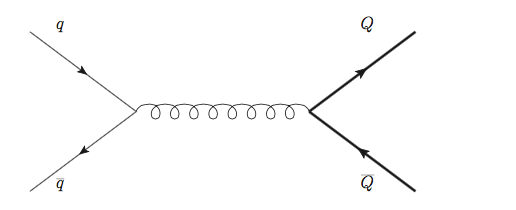
\includegraphics[width=8cm]{FigCap2/Feymann1.png}
  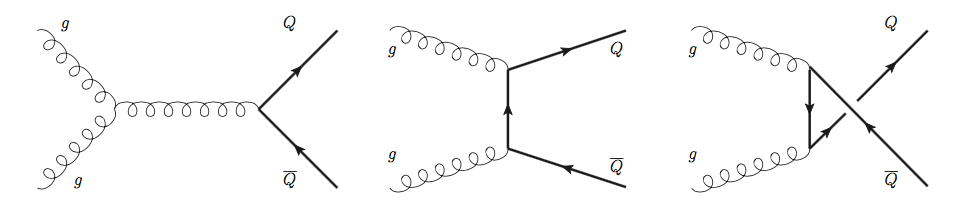
\includegraphics[width=15cm]{FigCap2/Feymann2.png}
  \caption{Leading-order diagrams for heavy-quark pair production.}
  \label{fig:LOdiagrams}
\end{figure}
\begin{figure}[!ht]
  \centering
  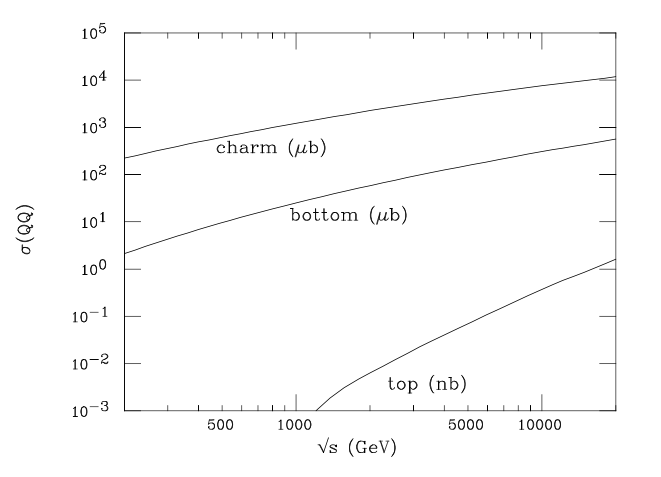
\includegraphics[width=7.6cm]{FigCap2/HQxsecPPcoll.png}
      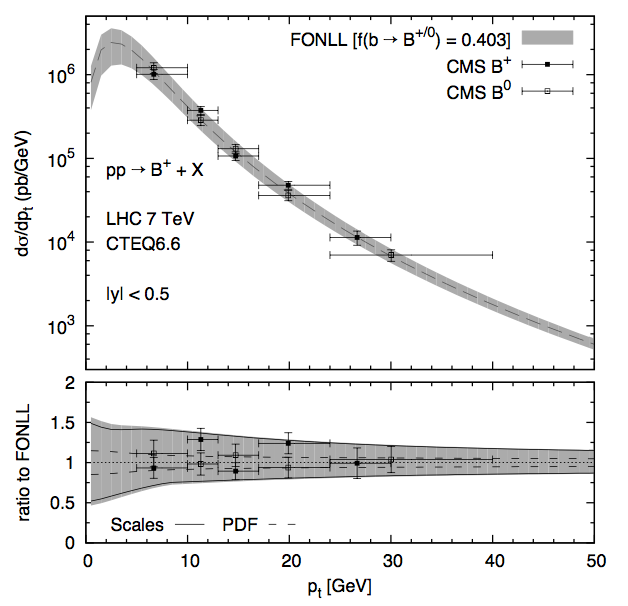
\includegraphics[width=6.4cm]{FigCap2/FONLLBmeson.png}
  \caption{Left: total production cross-sections for charm, bottom and top quark pairs, in pp collisions as a function of the center-of-mass energy~\cite{Mangano:1997ri}. Right: FONLL calculation and systematics band~\cite{Cacciari:2012ny} for beauty-hadron production, and comparison with CMS data~\cite{Khachatryan:2011mk,Chatrchyan:2011pw}, rescaled to the $|y| <$ 0.5 region.}
  \label{fig:HQxsecPPcoll}
\end{figure}
Analytic calculations that provide description for inclusive heavy hadron production or their decay products
in pp collisions are FONLL~\cite{Cacciari:1998it,Cacciari:2001td} and GM-VFNS~\cite{Kniehl:2004fy}. 
FONLL is a Fixed-Order plus Next-to-Leading-Logarithms 
calculation and provides predictions in the full kinematic range ($\pt \ll m_Q, \pt \sim m_Q, \pt \gg m_Q$),
giving description of bottom and charm production at Tevatron, RHIC and LHC. 
GM-VFNS was originally performed in the massless limit and subsequently improved with finite mass terms.
Within both models, the single inclusive distribution of a particle $l$ is obtained as a convolution of a
perturbative cross section $d\sigma$ with a non-perturbative fragmentation function $D^{NP}_{q->H_q}$
and possibly a decay function $g^{weak}_{H_q \rightarrow l}$ describing, for instance, the hadron weak decay into a lepton:
\begin{equation}
d\sigma_l = d\sigma_{q} \otimes D^{NP}_{q->H_q} \otimes g^{weak}_{H_q \rightarrow l}.
\end{equation}
The functional form of the non-perturbative fragmentation function (FF) $D^{NP}_{q->H_q}$ 
is generally chosen as result of fit on $e^+e^-$ data for heavy-hadron production. For example, FONLL uses
a Kartvelishvili et al.~distribution~\cite{Kartvelishvili:1977pi} for the FF of bottom quarks:
\begin{equation}
D^{NP}_{b->H_b}= (\alpha +1 )(\alpha +2)z^{\alpha} (1-z),
\end{equation}
where the fragmentation parameters $\alpha$ were chosen as a result of the fit~\cite{Cacciari:2005uk} on the LEP data concerning production
of a mixture of $b$-hadrons~\cite{Heister:2001jg,Abbiendi:2002vt}, since no data are available for individual hadrons like $B^0$ or $B^+$.
For charm quarks, experimental data for individual $\Dzero$, $\Dplus$, $\Dstar$, and $\Ds$ mesons exist.
Since from the theoretical point of view some discrepancies are known in the quark fragmentation into 
pseudo-scalar ($\Dzero, \Dplus$) and vector ($\Dstar$) mesons, one needs to define two different FF. One single non-perturbative parameter
describes both the scalar and vector FF, thus the parameter fitted to ALEPH data~\cite{Barate:1999bg} for $\Dstar$ production can
be used as input in the pseudo-scalar ($\Dzero$ and $\Dplus$) FF~\cite{Cacciari:2003zu}.
Fig.~\ref{fig:HQxsecPPcoll} (right) shows CMS measurement of $\pt$-differential cross-section for $B^+$ and $B^0$ mesons
as a function of $\pt$ with rapidity $|y| < 0.5$ at in pp collision at $\sqrt{s} = 7$ TeV~\cite{Khachatryan:2011mk,Chatrchyan:2011pw}, compared to FONLL predictions.
The FONLL uncertainty band is obtained from variations of renormalisation scale $\mu$ and common factorisation
scale $\mu_f$ as well as variations of the heavy-quark mass, added in quadrature.
Similar comparison but for charmed hadrons is in Fig.~\ref{fig:CharmXsec} for $\Dzero$-meson production
in pp collision at $\sqrt{s} = 7$ TeV measured by ALICE~\cite{Acharya:2017jgo}, as a function of $\pt$. FONLL predictions are displayed on the left panel and GM-VFNS on the right one. Calculations are in agreement with bottom and charm production at the LHC, within their
uncertainties. FONLL tends to underestimate charm production , in particular at low $\pt$, whereas GM-VFNS
tends to slightly overestimate them at high $\pt$ but agrees very well at intermediate-low $\pt$. \\



In contrast with FONLL and GM-VFNS, that are based on NLO calculations and are limited to inclusive production
of heavy quarks and mesons, general-purpose Monte Carlo generators provide a more complete description 
of the final state, including decay kinematics, particle identifications and even detector response. They simulate the 
final states of high-energy collisions in full detail and contain a large list of hard Standard Model and Beyond Standard Model processes, which are interfaced with parton emission, different models of hadronisation and particle decays. 
The processes are treated at leading order (LO). The higher order calculations are included only in an
approximate approach. However, the next-to-leading order (NLO) is needed to compare results with experimental data.
PYTHIA generator~\cite{Sjostrand:2006za}, for example, contains theoretical perturbative QCD calculations that are exact only
at leading order, where only the pair creation processes $q\bar{q} \rightarrow Q\bar{Q}$ and $gg \rightarrow Q\bar{Q}$
are included, and includes higher-order contributions at the NLO to account 
for flavour excitation processes like $qQ \rightarrow qQ$, $gQ \rightarrow gQ$
and the gluon splitting $g \rightarrow Q\bar{Q}$. The cross-section of these processes 
diverges as $\pt^{hard}$ goes to zero. The divergences can be controlled by a lower cut 
on the value of  $\pt^{hard}$, that has a large influence in the heavy-flavour production 
in the low-$\pt$ region, which is of the prime interest for ALICE. To compare PYTHIA to data, $\pt^{hard}$ and
other PYTHIA parameters must be tuned to reproduce as well as possible NLO predictions.
The first generator that did the effort of matching NLO calculations with LO calculations was MC@NLO~\cite{Frixione:2002ik}.
It proposed a first solution to the double counting of NLO events, by subtracting the approximated 
NLO cross section (which were implemented in the general generator) from the exact NLO cross section.
The NLO calculations for the hard processes are obtained within the POWHEG~\cite{Frixione:2007nw} (Positive Weight Hardest Emission Generator) method. 

\begin{figure}[!ht]
  \centering
  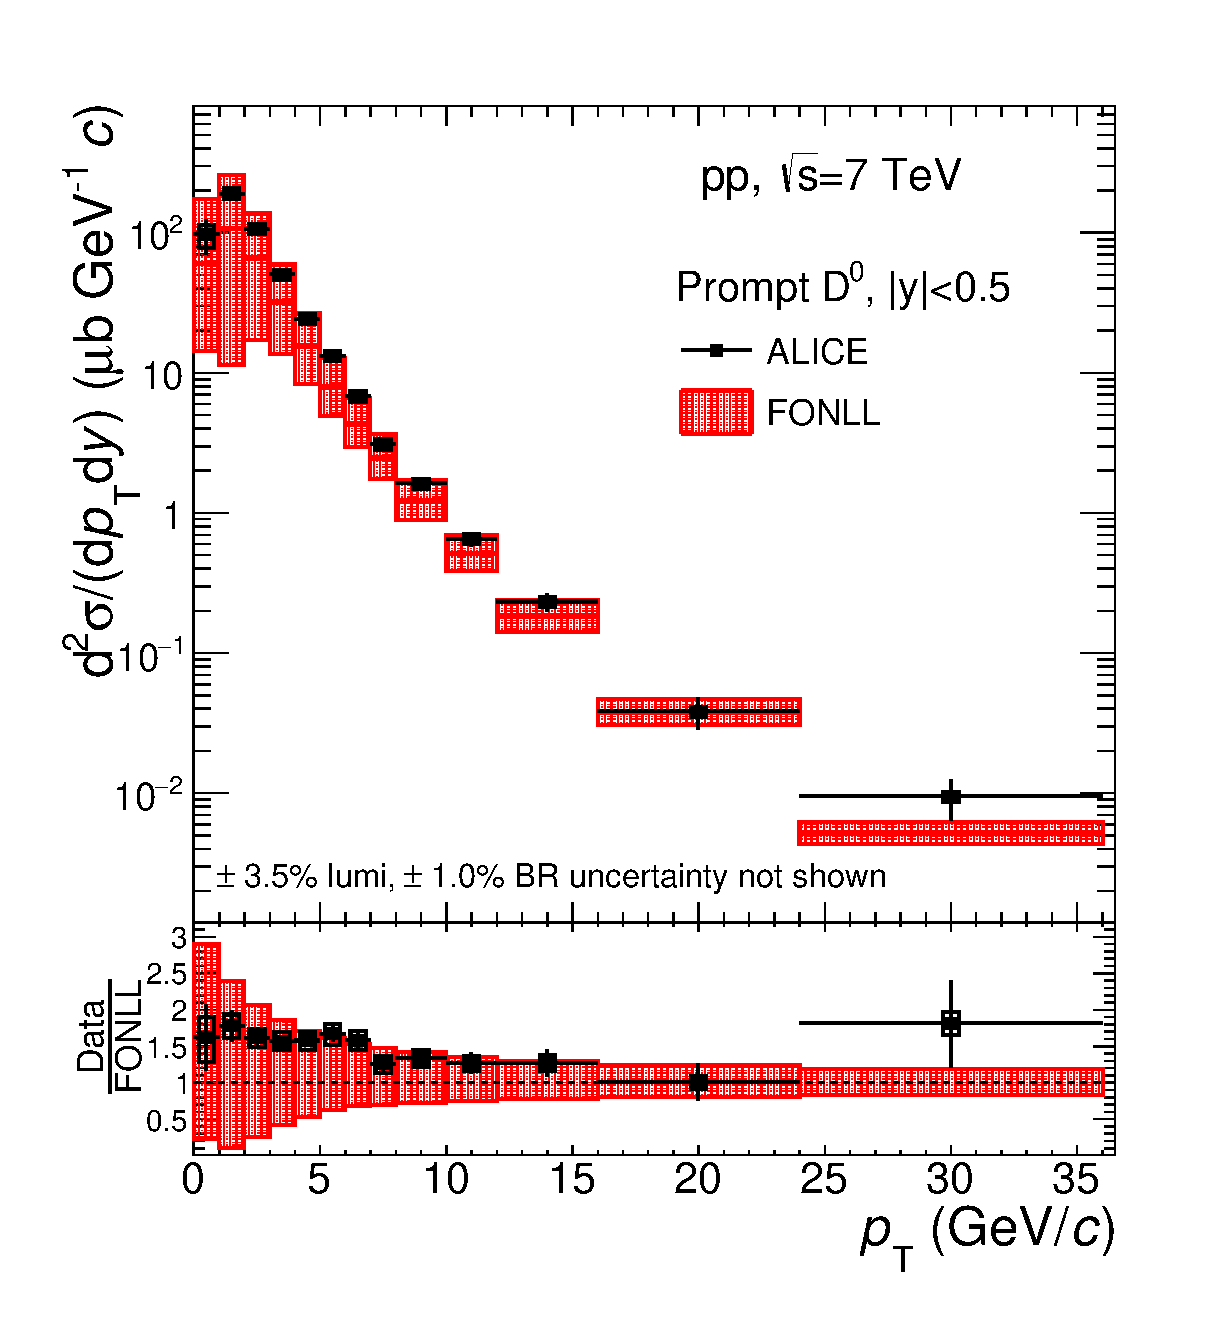
\includegraphics[width=7cm]{FigCap2/DzeroppCrossSecVsFONLLAndRatio.eps}
  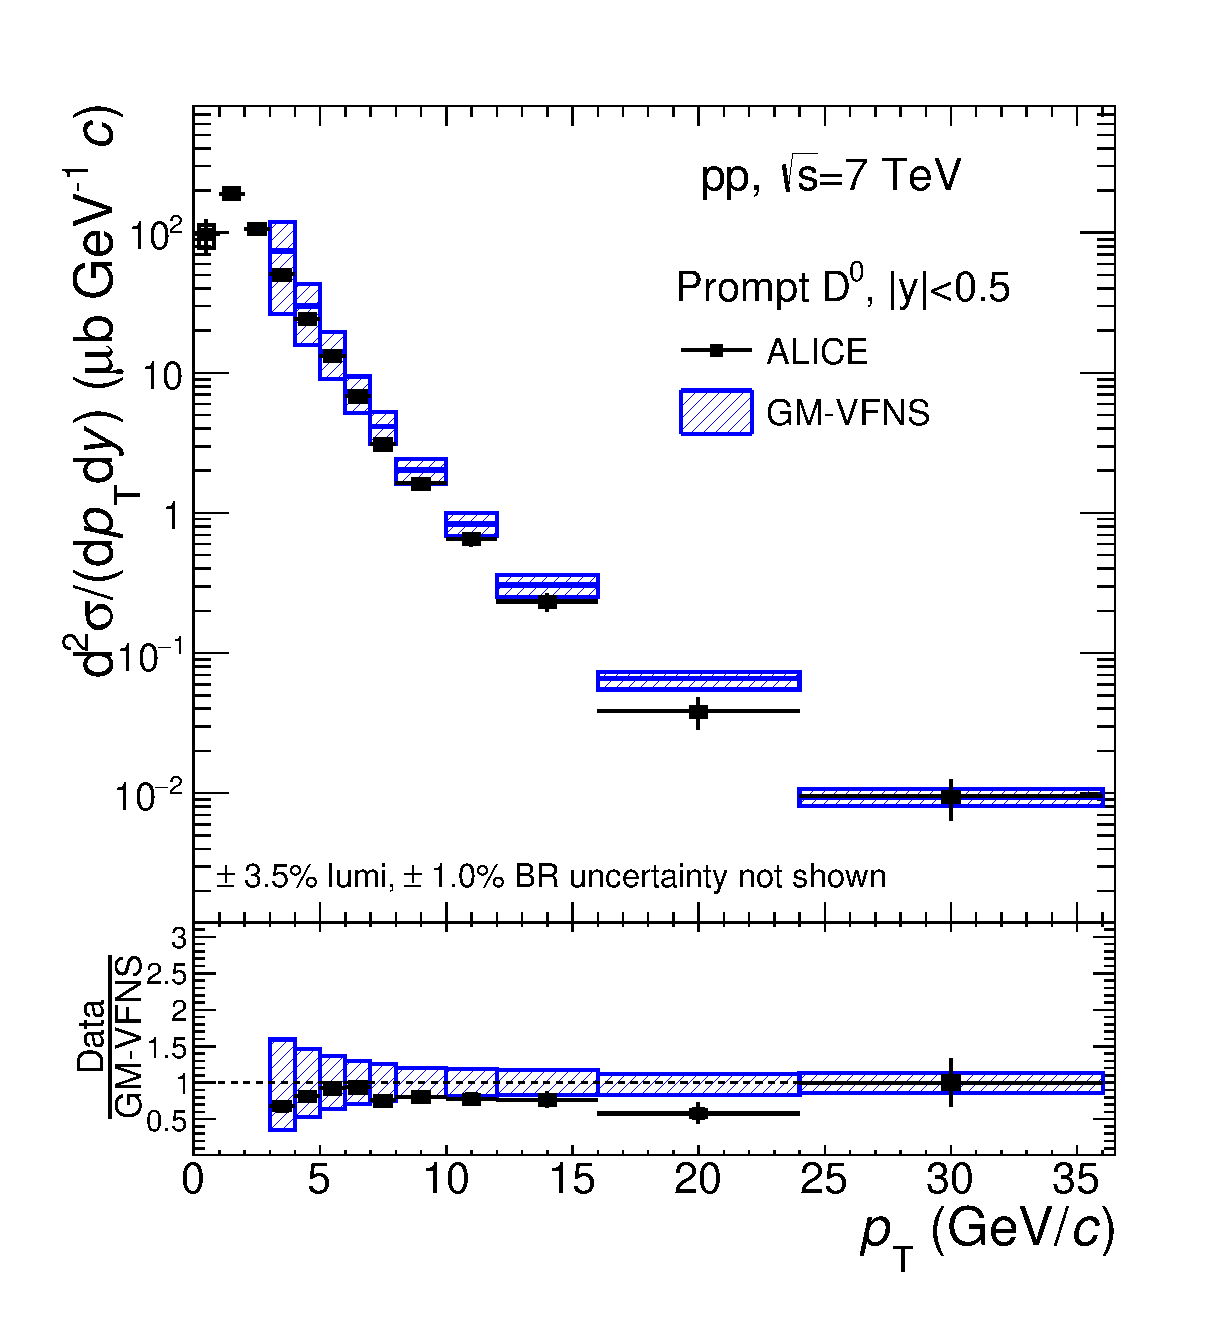
\includegraphics[width=7cm]{FigCap2/DzeroppCrossSecVsGMVFNSAndRatio.eps}
  \caption{$\pt$-differential production cross section of prompt $\Dzero$ mesons with $|y| < $ 0.5 in the interval $0 < \pt < 36 ~\Gevc$, in pp collisions at $\sqrt{s} = 7$ TeV~\cite{Acharya:2017jgo}. The cross section is compared to pQCD calculations: FONLL~\cite{Cacciari:1998it,Cacciari:2001td} (left panel) and GM-VFNS~\cite{Kniehl:2004fy} (right panel).}
  \label{fig:CharmXsec}
\end{figure}

\section{Heavy quarks in proton-nucleus collisions}
\subsection{Cold nuclear matter effects}
The importance of heavy flavours in p-A collisions relies on the possibility to
characterize a class of phenomena which are expected to break the binary scaling in 
nucleus-nucleus collisions but are not a consequence of the presence of a 
deconfined plasma. They can in fact be present both in p-A and in A-A collisions and
their origin is mainly related to nuclear PDFs. They are the so-called Cold Nuclear Matter (CNM) effects,
or initial-state effects.
Furthermore, recent interest in p-A collisions
is focused on revealing possible collective effects that could indicate presence of QGP in small systems.\\
One can define the nuclear modification factor $R_i^A(x,Q^2)$ for the parton distribution function:
\begin{equation}
\label{eq:RA}
R_i^A(x,Q^2) = f_{i/A}(x,Q^2) / f_{i/p}(x,Q^2)
\end{equation}
\begin{figure}[!ht]
  \centering
  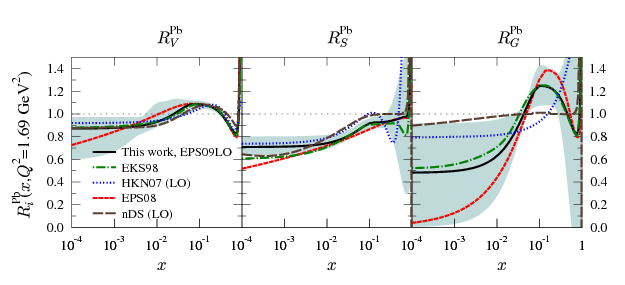
\includegraphics[width=15cm]{FigCap1/PartonNMF.png}
  \caption{The nuclear modification factor (Eq.~\ref{eq:RA}) in a Pb nucleus $R_i^A(x,Q^2)$ for three different flavours as given by the
available nPDF parametrization at LO~\cite{Eskola:2009uj}.}
  \label{fig:nPDF}
\end{figure}
where $f_{i/A}(x,Q^2)$ and $f_{i/p}(x,Q^2)$ are the parton distribution functions in the 
nucleus and in the proton respectively, and the variable $x$ represents the fraction of 
the nucleon momentum carried by a parton. Fig.~\ref{fig:nPDF} 
shows nuclear modification factors $R_i^A(x,Q^2)$ for the valence quarks, sea quarks and 
gluons inside a Pb nucleus from LO global DGLAP calculations EKS98~\cite{Eskola:1998df,Eskola:1998iy}, 
EKPS~\cite{Eskola:2007my},
nDS~\cite{Eskola:2008ca}, HKN07~\cite{Hirai:2007sx} and EPS09LO~\cite{Eskola:2009uj}. 
In general, four different regions are visible in the trend of $R_i^A(x,Q^2)$ versus $x$,
which correspond to four $x$-regimes. The effects that are related to these regions are typically referred to as:
\begin{itemize}
\item {\bf Fermi motion ($x > 0.7$):} dominating the region of valence quarks, this effect is due to the 
thermal momentum that nucleons have inside the nucleus. Thus the structure function $F^A_2(x)$ of the nucleus
is the convolution of the structure function of the nucleon with the momentum distribution
of nucleons $f_N(z)$ inside the nucleus: $F^A_2(x) = \int_x^A dz f_N(z) F_2^N(x/z)$, where $z$ is the momentum fraction
of the nucleons times the atomic number of the nucleus.
\item {\bf EMC effect ($0.2 < x < 0.7$):} first observed in 1982 by EMC collaboration~\cite{Aubert:1983xm},
this effect implies a depletion of the  $R_i^A(x,Q^2)$ still in the region of valence quarks (see Fig.~\ref{fig:EMC} left), where one would expect 
the ratio of the structure functions of iron $F^{iron}_2(x)$ and deuterium $F^D_2(x)$ to be at 1 (except for 
some corrections at high $x$ from Fermi motion). From further
experimental investigations, it was clear that the effect had a universal shape, was independent of the 
squared momentum transfer, increased with nuclear mass number A and scaled with the average nuclear density. 
Many phenomenological models tried to explain the reason of such behaviour. In the simplest model, 
quarks in nuclei move in a larger confinement volume and, because of the uncertainty principle, 
they carry less momentum than quarks in free nucleons. Some models proposed that 
quarks in nuclei move in quark bags with $n$ quarks, other proposed an enhancement 
of pion-cloud effects and a nuclear pionic field, but no models so far are universally accepted. 
 In 2009 other pieces of information were added with the
discover of a strong correlation between the slope in the region of EMC effect and the magnitude of the scaling plateau 
at $x > 1$ (see Fig.~\ref{fig:EMC}, right panel)~\cite{Seely:2009gt}.
\item {\bf Nuclear shadowing region ($x < 0.01$):} a second depletion region
is observed in the ratio of structure functions $R_i^A(x,Q^2)/R_i^D(x,Q^2)$ at very low $x$ (typical region of sea quarks), and
an {\bf anti-shadowing region} at $0.01 < x < 0.2$ between shadowing and EMC region.~Different solutions were
proposed to explain the nuclear shadowing. Some models are based on virtual photon fluctuations (GVMD); others
describe a superposition of partons of different nucleons, that should deplete the parton region at low $x$, thus favouring
the creation of the anti-shadowing region.

\end{itemize}


\begin{figure}[!ht]
  \centering
  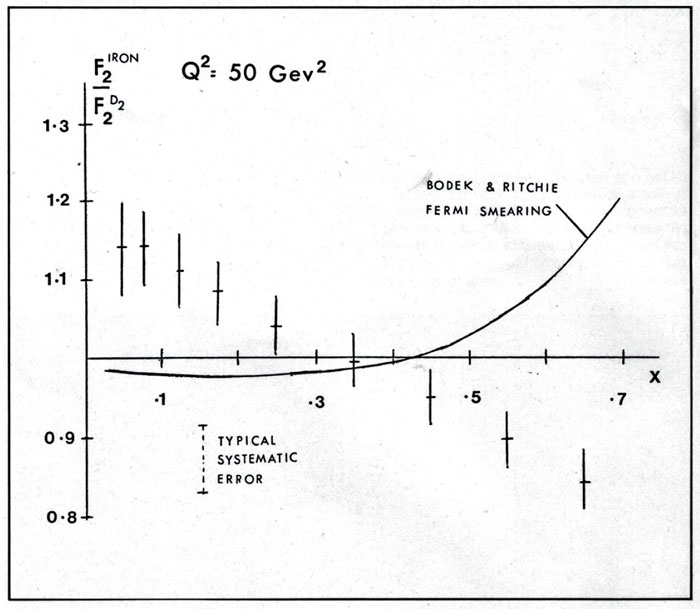
\includegraphics[width=6.5cm]{FigCap2/EMC.jpg}
  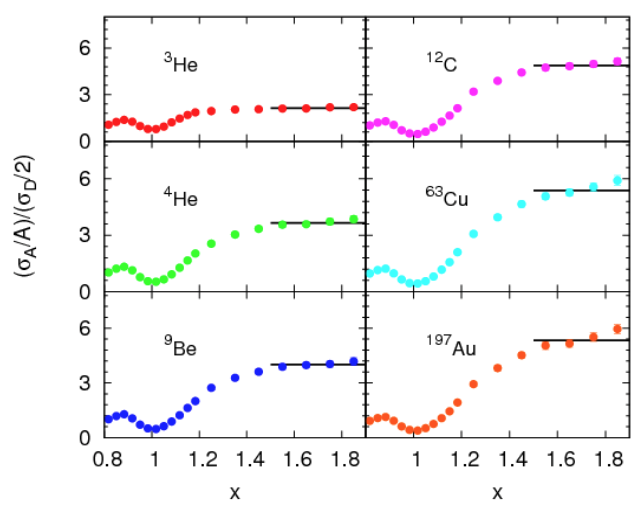
\includegraphics[width=7.5cm]{FigCap2/EMC2.png}
  \caption{Left: ratio of iron $F^{iron}_2(x)$ and deuterium $F^D_2(x)$ structure function as a function of Bjorken-$x$~\cite{Aubert:1983xm}. Right: ratio of nucleus $F^{A}_2(x)$ and deuterium $F^D_2(x)$ for different nuclei as a function of Bjorken-$x$~\cite{Seely:2009gt}.}
  \label{fig:EMC}
\end{figure}



An other mechanism which must be cited among the CNM effects, still having nothing to do with nuclear PDF modification, is the Cronin Effect~\cite{Cronin:1974zm}, discovered in the ’70s at FermiLab. It is responsible for an enhancement in the nuclear modification factor for $\pt$ values between 2 and 5 $\Gevc$. In p-A collisions, the nucleon traversing the nucleus undergoes several elastic scatterings with the partons before the hard scattering process occurs. The multiple scatterings give the parton an extra momentum component in the transverse plane ($k_{\rm T}$ broadening), which causes a broadening of the $\pt$ spectra of the heavy quarks produced in the hard scattering processes, providing one possible explanation to the enhancement.~Going towards even larger values of transverse momentum, the extra-$k_{\rm T}$ from the elastic collisions becomes negligible and the nuclear modification factor gets close to 1 again.\\
%The x regime relevant for charm production at the LHC ($\sim 10^{-4}$ ) is about 2 orders of magnitude lower than at RHIC and 3 orders of magnitude lower than at the SPS [43]. In this region with low x-values, modifications of the nuclear PDFs are mainly related to the shadowing effect.
\begin{figure}[!ht]
  \centering
  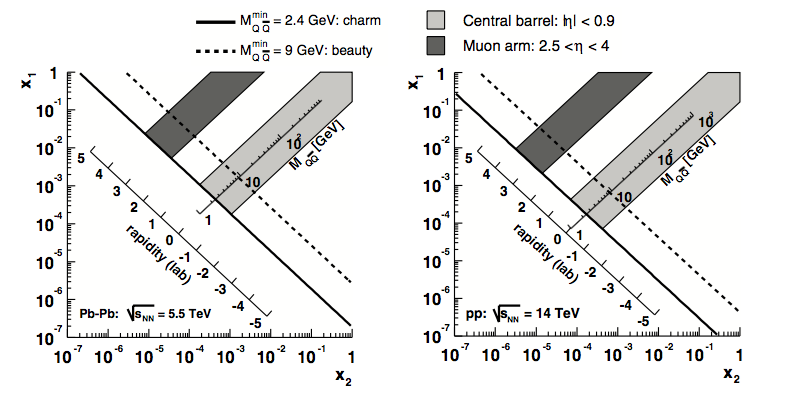
\includegraphics[width=15cm]{FigCap2/xBjork.png}
  \caption{ALICE acceptance in the ($x_1, x_2$) plane for heavy flavours in Pb-Pb at $\sNN = 5$ TeV on the left panel and pp collisions at $\sqrt{s} = 14$ TeV on the right~\cite{Alessandro:2006yt}. }
  \label{fig:xBjork}
\end{figure}



Let's turn now to understand which are the ranges of Bjorken $x$
at play when producing $c\bar{c}$ and $b\bar{b}$ pairs at the LHC and which are the
variables that control $x$ values. The probed $x$ value depends indeed on the center-of-mass energy
of the collision, on the invariant mass $M_{Q\bar{Q}}$ of the $Q\bar{Q}$ pair produced in the hard scattering
and on its rapidity $y_{Q\bar{Q}}$. Under the hypothesis that the transverse momentum of the parton 
in the nucleon is negligible, the four-momenta of the two incoming gluons are $(x_1,0,0,x_1)\cdot(Z_1/A_1)\sqrt{s_{\rm pp}}/2$
and $(x_2,0,0,-x_2)\cdot(Z_2/A_2)\sqrt{s_{\rm pp}}/2$, with $x_1$ and $x_2$ are the momentum fractions 
carried by the gluons, and $\sqrt{s_{\rm pp}}$ is the c.m.s. energy for pp collisions. 
The square of the invariant mass of the $Q\bar{Q}$ pair is given by:
\begin{equation}
\label{eq:Mqq}
M_{Q\bar{Q}}^2 =  x_1 x_2 s_{\rm NN} = x_1 \frac{Z_1}{A_1} x_2 \frac{Z_2}{A_2} s_{\rm pp},
\end{equation}
and the rapidity in the laboratory is:
\begin{equation}
\label{eq:yqq}
y_{Q\bar{Q}} = \frac{1}{2} {\rm ln} {\Big [ } \frac{E +p_z}{E-p_z}  {\Big ] }= \frac{1}{2} {\rm ln} {\Big [ } \frac{x_1}{x_2} \cdot \frac{Z_1 A_2}{Z_2 A_1} {\Big ] }.    
\end{equation}
From Eq.~\ref{eq:Mqq} and~\ref{eq:yqq} and for a symmetric colliding system $(A_1 = A_2, Z_1 = Z_2)$
one obtains:
\begin{equation}
\label{eq:x1x2}
x_1 = \frac{M_{Q\bar{Q}}}{\sqrt{s_{\rm NN}}} {\rm exp} (+y_{Q\bar{Q}} ), \; \; \; \; \; \;
x_2 = \frac{M_{Q\bar{Q}}}{\sqrt{s_{\rm NN}}} {\rm exp} (-y_{Q\bar{Q}} ). 
\end{equation}
Because of its lower mass, charm allows one to probe lower $x$ values than beauty. 
The $x$ regime relevant for charm production at the LHC ($\approx 10^{-4}$) is about 
2 orders of magnitude lower than at RHIC and 3 orders of magnitude lower than at the SPS.
Measurements of charm and beauty particles in the forward (or backward) rapidity region ($|y| \sim 4 $) 
gives access to $x$ regimes about 2 orders of magnitude lower, down to $x \approx 10^{-6}$.
Fig.~\ref{fig:xBjork}~\cite{Alessandro:2006yt} shows the ($x_1, x_2$) plane for charm and bottom production at the LHC
covered by ALICE acceptance, for Pb-Pb
collisions at $\sNN = 5$ TeV on the left panel and pp collisions at $\sqrt{s} = 14$ TeV on the right.
The shadowed regions correspond to the rapidity region covered by the ALICE barrel ($|\eta| < 0.9$) and by the 
muon arm ($-4 < \eta < -2.5$).
The points with equal invariant mass ($c\bar{c}$ and $b\bar{b}$ pairs) lie on hyperbolae (straight lines in the log-log scale).\\


\subsection{Experimental results in pA}
The modifications of PDFs at small $x$ can significantly reduce final hadrons yields.
One can define the nuclear modification factor for p-Pb collisions as:
\begin{equation}
R_{\rm pPb} = \frac{1}{A}\frac{d^2\sigma_{pPb}^{\rm prompt D}/d\pt dy}{d^2\sigma_{pp}^{\rm prompt D}/d\pt dy},
\end{equation}
where A is the Pb mass number $A = 208$. \\
\begin{figure}[!ht]
  \centering
  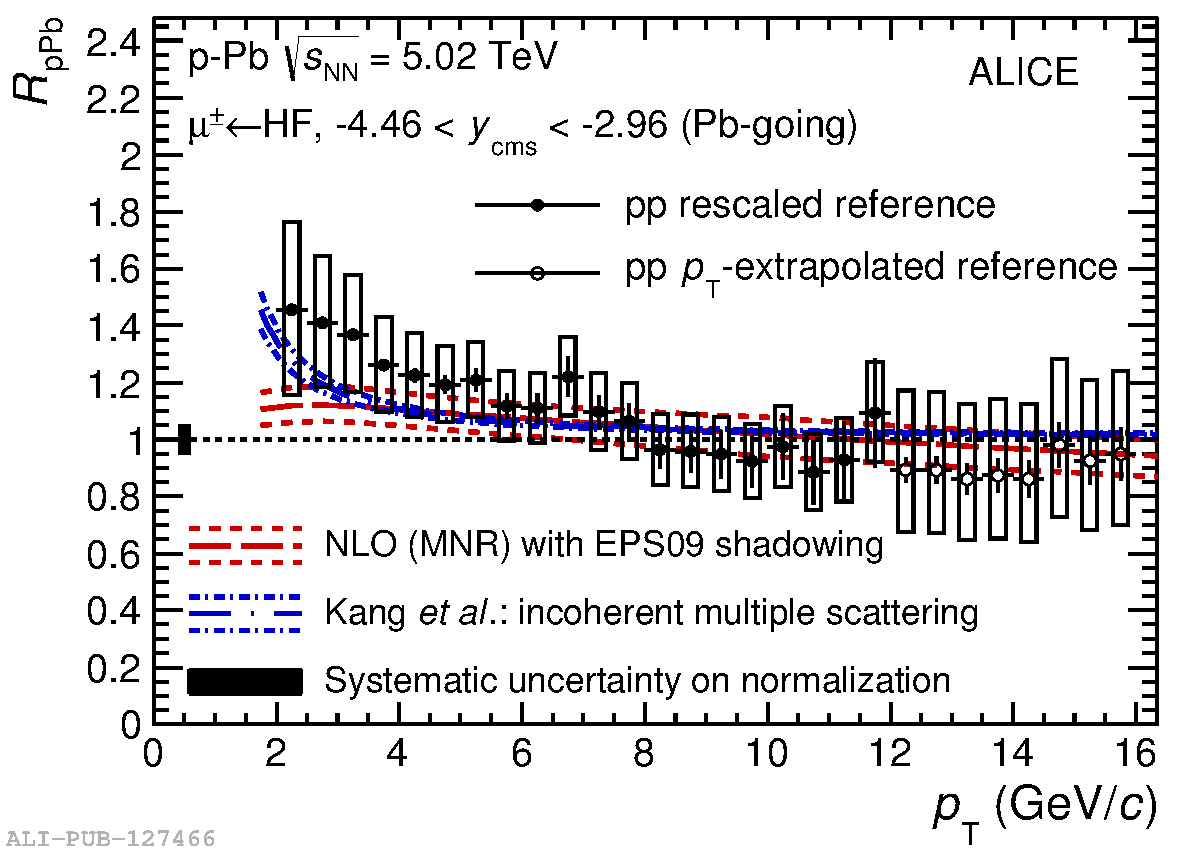
\includegraphics[width=7cm]{FigCap2/2017-Feb-05-Fig2b.pdf}
  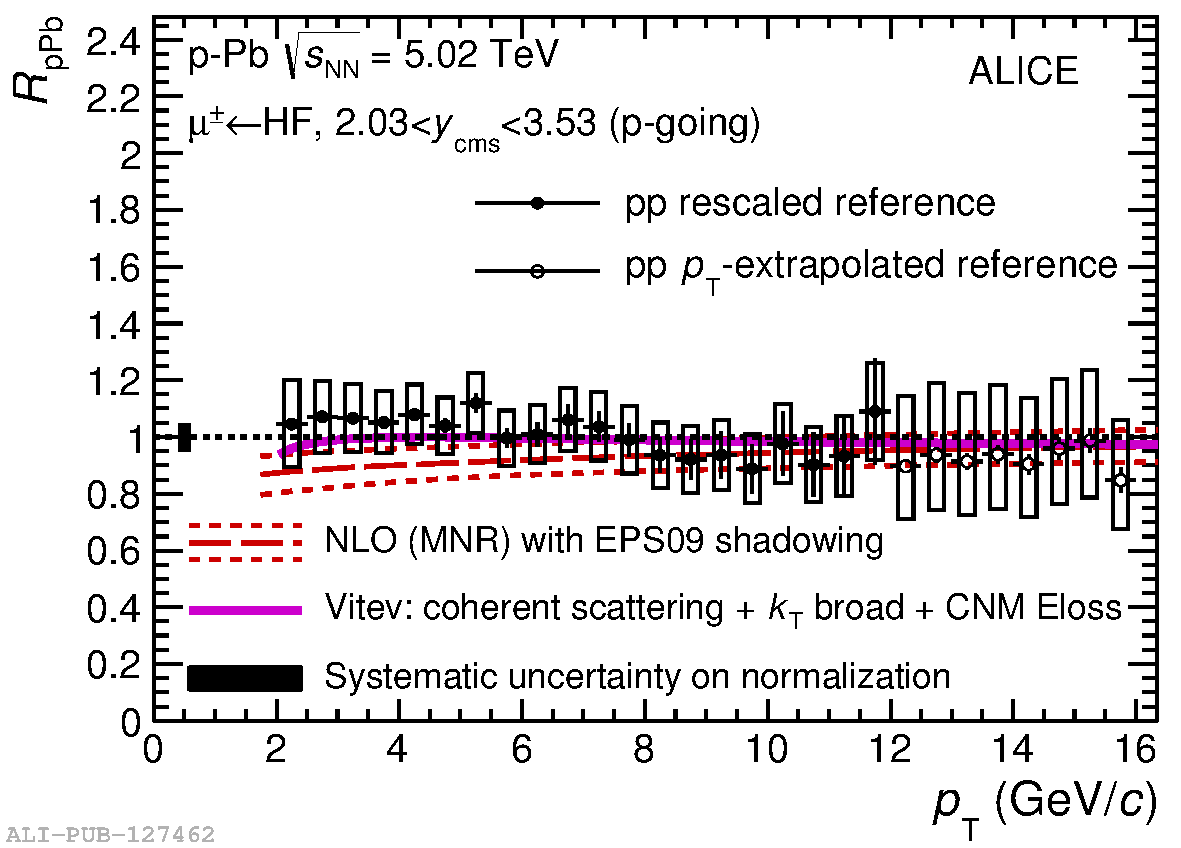
\includegraphics[width=7cm]{FigCap2/2017-Feb-05-Fig2a.pdf}
  \caption{Nuclear modification factor of muons from heavy-flavour hadron decays as a function of $\pt$ for p-Pb collisions at $\sNN = 5.02$ TeV at backward rapidity ($4.46 < y_{\rm cms} < 2.96$, left) and forward rapidity ($2.03 < y_{\rm cms} < 3.53$, right)~\cite{Acharya:2017hdv} compared to model predictions~\cite{Kang:2014hha,Mangano:1991jk}. }
  \label{fig:muons}
\end{figure}
\begin{figure}[!ht]
  \centering
    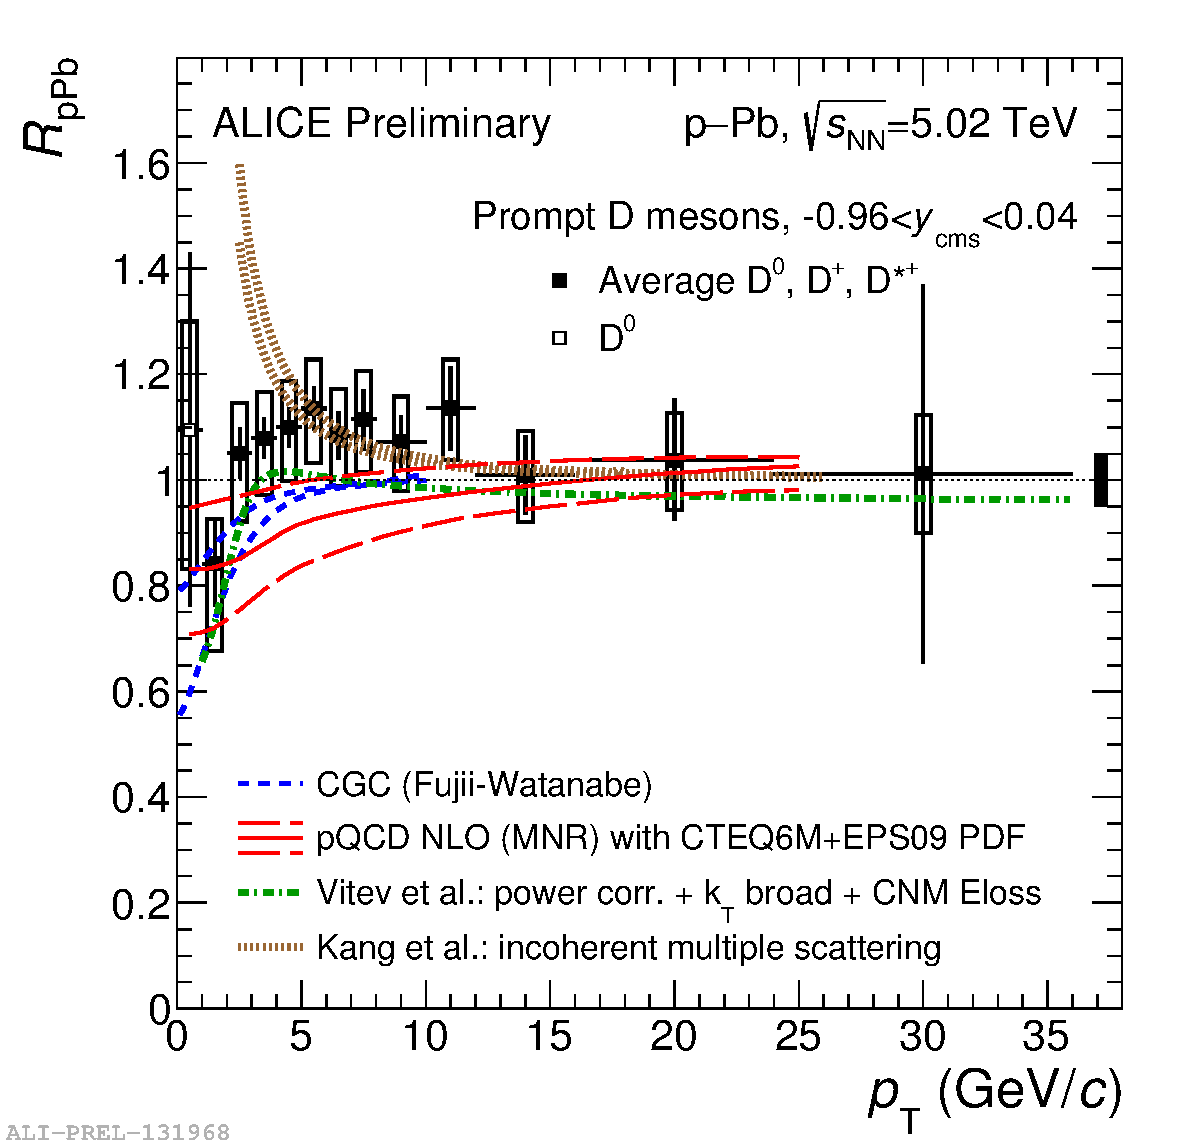
\includegraphics[width=7cm]{FigCap2/2017-Jul-05-pPbWithModelsCNM.pdf}
    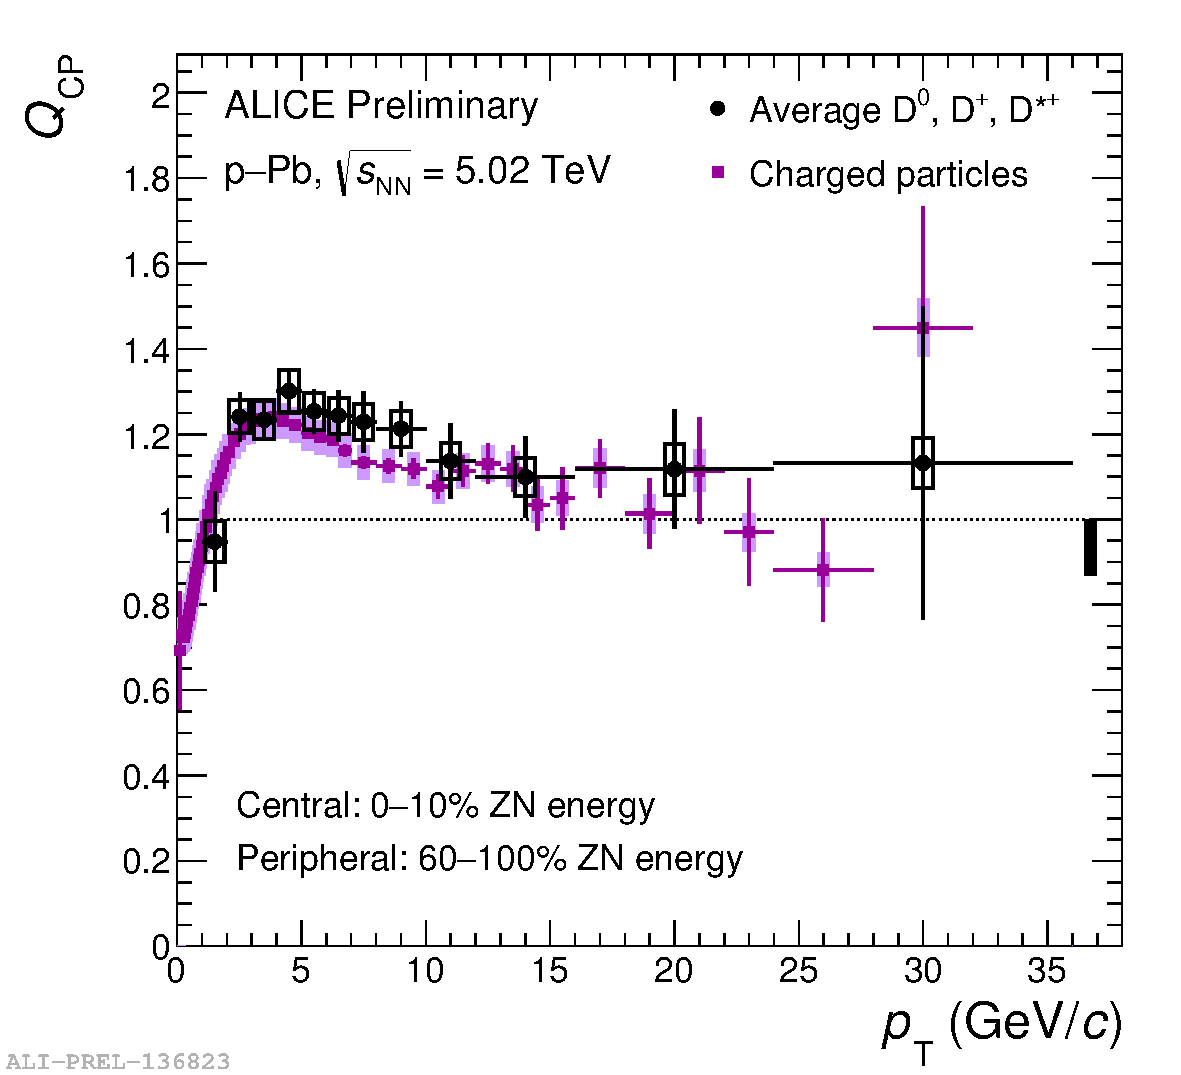
\includegraphics[width=7cm]{FigCap2/2017-Sep-12-QCP-Daverage-ChargedHadrons.pdf}
  \caption{Left: nuclear modification factor $R_{\rm pPb}$ of prompt D mesons in p-Pb collisions at $\sNN = 5.02$ TeV. Data are compared with results of theoretical calculations including only CNM effects~\cite{Fujii:2017rqa,Cacciari:2012ny,Eskola:2016oht,Sharma:2009hn,Kang:2014hha}. Right: $\Dzero$ (black) and charged-particle (magenta) central-to-peripheral nuclear modification factor~\cite{ALICEPAS2017008}.}
  \label{fig:RpA}
\end{figure}


ALICE measured the $\pt$-differential $R_{\rm pPb}$ of muons from heavy-flavour hadron decays in p-Pb collisions at $\sNN = 5.02$ TeV
at forward and backward rapidity~\cite{Acharya:2017hdv} (Fig.~\ref{fig:muons}).
While at forward rapidity muon $R_{\rm pPb}$ is compatible with unity in the full $\pt$ range, 
at backward rapidity, it is larger than unity with a maximum 
significance of 2.2$\sigma$ of the combined statistical and systematic uncertainties in the interval $2.5 < \pt < 3.5 \;\Gevc$. 
At higher $\pt$, it is compatible with unity. The results indicate
that CNM effects are small and that the strong suppression of the
yields of muons from heavy-flavour hadron decays observed in the
10\% most central Pb-Pb collisions~\cite{Abelev:2012qh} should result from final-state
effects, e.g. the heavy-quark in-medium energy loss. 
ALICE also measured $R_{\rm pPb}$ of prompt D mesons in p-Pb collisions at $\sNN = 5.02$ TeV
as a function of $\pt$ and results are shown in Fig.~\ref{fig:RpA} (left panel)~\cite{ALICEPAS2017008}. Data are compared to 
theoretical models that include CNM effects. In general, calculations describe the data within 
uncertainties in the entire $\pt$ range. CNM effects are expected to be largest for small $\pt$, 
where, in addition, the predictions of the different theoretical approaches differ and the statistical 
uncertainty of the present measurement for the lowest $\pt$ interval is about 30\% and does not 
allow to draw a conclusion. \\

One can also define the nuclear modification factor in p-Pb collisions in given centrality classes, as:
\begin{equation}
Q_{\rm pPb}^{\rm cent} = \frac{(\der^2 N^{\rm prompt D }/\der \pt \der y)^{\rm cent}_{\rm pPb}}{\langle T_{\rm pPb} \rangle ^{\rm cent}(\der^2 \sigma^{\rm prompt D }_{pp}/\der \pt \der y)},
\end{equation}
where $(\der^2 N/\der \pt \der y)^{\rm cent}_{\rm pPb}$ is the yield of prompt D mesons in p-Pb collisions 
in a given centrality class, and $\langle T_{\rm pPb} \rangle ^{\rm cent}$ is the average nuclear overlap function in a given centrality class.
Finally, the ratio of the nuclear modification factor in central to peripheral events, $Q_{\rm CP}$, 
can be defined in order to achieve better precision on the yields:
\begin{equation}
Q_{\rm CP} = \frac{(\der^2 N^{\rm prompt D }/\der \pt \der y)^{\rm central}_{\rm pPb}/ \langle T_{\rm pPb} \rangle^{central}}{(\der^2 N^{\rm prompt D }/\der \pt \der y)^{\rm peripheral}_{\rm pPb}/ \langle T_{\rm pPb} \rangle^{peripheral}}.
\label{eq:QCP}
\end{equation}
The $Q_{\rm CP}$ of D mesons in the 0-10\% and 60-80\% centrality classes was measured by 
ALICE~\cite{ALICEPAS2017008} (Fig.~\ref{fig:RpA}, right panel) and it increases in the interval 1-4 $\Gevc$, 
up to values of about 1.25 and then tends to decrease. The average value of the D-meson $Q_{\rm CP}$ 
in the interval $3 < \pt < 8 \Gevc$ is larger than unity by 1.5 standard deviations of the combined statistical and systematic uncertainty.
It is an open question whether the observed bump of $Q_{\rm CP}$, whose magnitude is similar 
for D mesons and charged particles, is related to initial state effects or any collectivity effects.

\begin{figure}[!ht]
  \centering
  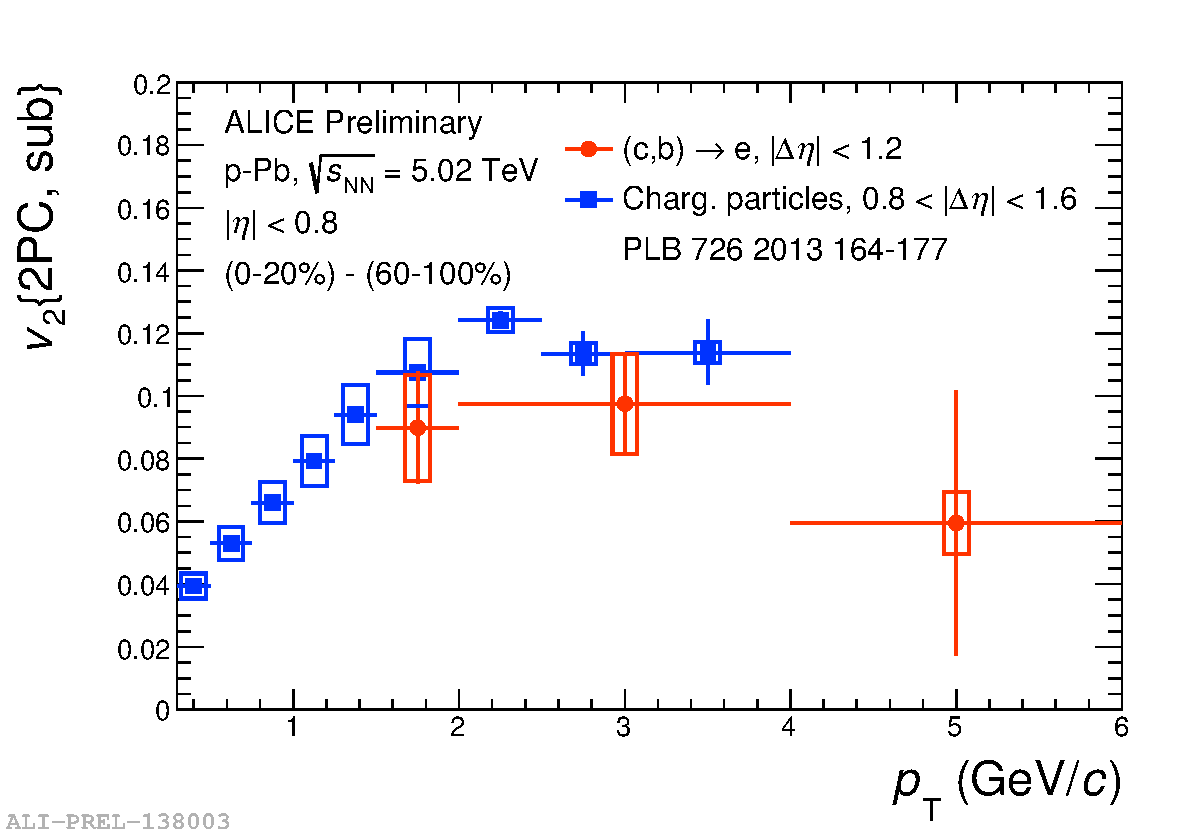
\includegraphics[width=7cm]{FigCap2/v2HFE.pdf}
  \caption{~\cite{Acharya:2017hdv}}
  \label{fig:}
\end{figure}

\section{Energy loss in AA collisions}
High-momentum partons traversing the QGP are expected to quench because of interactions 
with the medium constituents. The experimental observable used for the study of energy loss is the 
nuclear modification factor, defined in Sec.~\ref{sec:JetQuenching}. The possibility of disentangling
effects of cold nuclear matter from the ones related to in-medium energy loss paves the way to characterise the 
medium properties. In fact, in-medium interactions are connected to properties of the fireball like the transport coefficients,
that encode the momentum transfers with the medium, or the mean free path, closely related to the medium density $\rho$
and the cross section $\sigma$ of the parton-medium interaction. Depending on the kinematic region, a colour charge 
can lose energy in a plasma with temperature $T$ by two mechanisms: radiative and collisional energy loss.
\subsection{Collisional processes}
Collisional processes are $2 \rightarrow 2$ elastic scatterings off thermal quarks (Fig.~\ref{fig:LoopCollScatt}, first diagram) and gluons (Fig.~\ref{fig:LoopCollScatt}, second to fourth diagrams). It is possible to calculate, in the limit $E \gg M^2/T$, the heavy-quark collisional energy loss $\der E/\der x$ in a QGP, by summing all contributions~\cite{Peigne:2008nd}:
\begin{equation}
\label{eq:QCDenLossColl}
\begin{split}
\frac{\der E}{\der x} = \; & \frac{4 \pi T^2}{3}\;  \alpha_s (m^2_D)\;  \alpha_s(ET) {\Big [} {\Big (}  1 + \frac{n_f}{6}{\Big )} {\rm ln} \frac{ET}{m^2_D} + \frac{2}{9} \frac{\alpha_s(M^2)}{\alpha_s(m^2_D)} \times {\rm ln} \frac{ET}{M^2}  \\+\;  &c(n_f) + \mathcal{O}{\Big (}\alpha_s (m^2_D) \; {\rm ln}\frac{ET}{m^2_D}{\Big )}{\Big ]},
\end{split}
\end{equation}
where $\alpha_s$ is the QCD running coupling constant, $n_f$ is the number of flavours 
considered in the scattering diagrams of Fig.~\ref{fig:LoopCollScatt} and $m_D$ is the 
Debye screening mass of the plasma $m_D = 4\pi \alpha_s T^2 (1 + n_f/6)$. 
\begin{figure}[!ht]
  \centering
  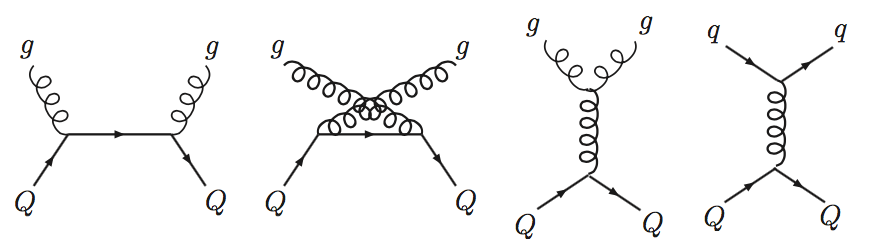
\includegraphics[width=14cm]{FigCap2/LO_HQscattering.png}
  \caption{Feynman diagrams for leading-order perturbative HQ scattering off light partons.}
  \label{fig:LoopCollScatt}
\end{figure}

The multiple scatterings of the heavy quark with the medium partons can also be treated as Brownian motion and typically
be described by Boltzmann equation. In the limit of small momentum transfer, the latter can be reduced to 
Fokker-Planck equation, which is often further reduced into Langevin equation. These
partial-differential equation can be used as transport equation, to give the evolution of the momentum distribution
of heavy quarks along time. The Langevin equation for heavy-quark collisional energy loss presents itself as~\cite{Cao:2013ita}:
\begin{equation}
\label{eq:Langevin}
\frac{{\rm d} {\vec{p}}}{\der t} = - \eta_D (p) \vec{p} + \vec{\xi}.
\end{equation}
In Eq.~\ref{eq:Langevin}, the first right-hand side term is the collision term, while the second one is the thermal random force,
satisfying the properties:
\begin{equation}
\label{eq:Langevin2}
\langle {\xi^i (\pt)} {\xi^j (p_{\rm T'})} \rangle = b^{ij} (\pt) \frac{\delta_{tt'}}{\der t}, \; \; \; \; b^{ij} (\pt) = k_{\parallel}(p)\hat{p}^i\hat{p}^j + k_{\perp} (\delta^{ij} - \hat{p}^i\hat{p}^j).
\end{equation}
In Eq.~\ref{eq:Langevin2}, $k$ represents the momentum space diffusion coefficient of heavy quarks;
$\eta_D$ is involved in the definition of the spatial diffusion coefficient D, which is related to the momentum space 
diffusion coefficient via: 
\begin{equation}
\label{eq:Langevin3}
D = \frac{T}{M \eta_D} = \frac{2 T^2}{k}.
\end{equation}
To simulate the evolution of heavy quarks, one needs to discretise terms and calculate the increment 
$\vec{p}(t + \Delta t) -  \vec{p}(t)$. 

\subsection{Gluon-radiative processes}
While a parton is traversing the medium, it picks up some transverse momentum $k_{\perp}$ due to multiple scatterings. 
If we consider a gluon in the hard parton wave function, when the accumulated $k_{\perp}$ is enough, it can decohere from the partonic projectile and be emitted.
These are $1 \rightarrow 2$ processes, like $Q \rightarrow g\, Q$, where $Q$ is the heavy quark and $g$ the gluon.
The average phase $\phi$ of the gluon is approximately:
\begin{equation}
\label{eq:gluonPhase}
\phi = {\Big \langle} \frac{k_{\perp}^2}{2\omega} \Delta z {\Big \rangle} \sim \frac{\hat{q} L}{2 \omega} L = \frac{\omega_c}{\omega},
\end{equation}
where $\hat{q}$ is the transport coefficient of the medium, defined as the average squared transverse 
momentum transferred to the projectile per unit path length $L$, $\hat{q} = \langle k_{\perp}^2 \rangle / L$ \cite{Salgado:2003gb,}.
Hence, gluons are emitted from the parton traversing a finite path length L with a characteristic gluon frequency $\omega_c$:
\begin{equation}
\label{eq:gluonPhase}
\omega_c = \frac{1}{2} \hat{q} L^2.
\end{equation}
The distribution of energy $\omega$ of the radiated gluons, for small energies $\omega < \omega_c$ is of the form:
\begin{equation}
\label{eq:gluonEnDistrb}
\omega \frac{\der I}{\der \omega} \sim \frac{2 \alpha_s C_R}{\pi} \sqrt{ \frac{\omega_c}{2 \omega}},
\end{equation}
where $C_R$ is the Casimir factor for the QCD coupling, equal to 4/3 for quark-gluon coupling and to 3 for gluon-gluon coupling.
The $\omega$-integrated average parton energy loss is then calculable from:
\begin{equation}
\label{eq:RadEnLoss}
\langle \Delta E \rangle = \int_0^\infty \der \omega \, \omega \frac{\der I}{\der \omega} \propto \alpha_s \, C_R \, \omega_c \propto \alpha_s \, C_R \, \hat{q} \, L^2. 
\end{equation}
We can then summarise the main properties of average parton energy loss via radiative processes:
\begin{itemize}
\item it grows like: $\Delta E \propto L^2$;
\item is proportional to $\alpha_s C_R$, thus it is larger by a factor 9/4 $ = 2.25$ for gluon-gluon than for quark-gluon processes;
\item it is independent of the initial parton energy $E$.
\end{itemize}
Furthermore, while in the limit of massless partons the probability of gluon emission is maximum for collinear radiation,
in the massive limit, the soft-gluon emission probability, for small emission angles $\Theta \ll 1$ is~\cite{Dokshitzer:1991fd}:
\begin{equation}
\label{eq:DeadCone}
\der \sigma_{Q \rightarrow Q + g} \sim \frac{\Theta^2 \der \Theta^2}{[\Theta^2+ \Theta^2_0]} \frac{\der \omega}{\omega}.
\end{equation}
Therefore, in the kinematical region $\Theta < \Theta_0$ the yield of radiated gluons
in the forward direction provides a small contribution to the total multiplicity. The depleted forward region is called the {\it dead cone}.
Since $\Theta_0 = M_Q/E_Q$, the effect is expected to be more relevant with increasing parton mass. A hierarchy in 
the energy loss is hence expected:
\begin{equation}
\label{eq:HierachyRaa}
\Delta E_{gluon} < \Delta E_{lightquark} < \Delta E_{heavyquark},
\end{equation}
where the first inequality comes from the Casimir factor and the second from the dead-cone effect. The hierarchy, if present, 
should consequently affect the $\RAA$.\\


\begin{figure}[!ht]
  \centering
  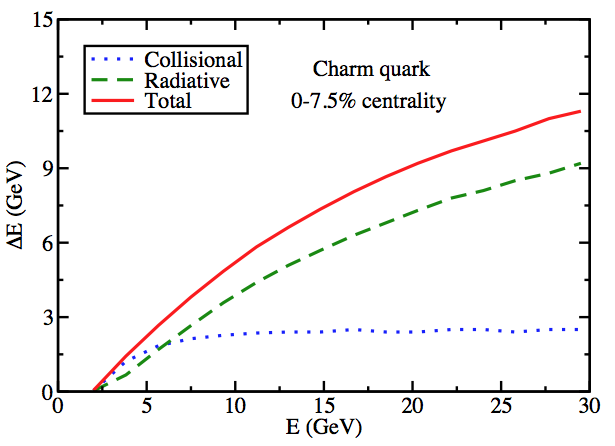
\includegraphics[width=7cm]{FigCap2/HFEnLoss1.png}
  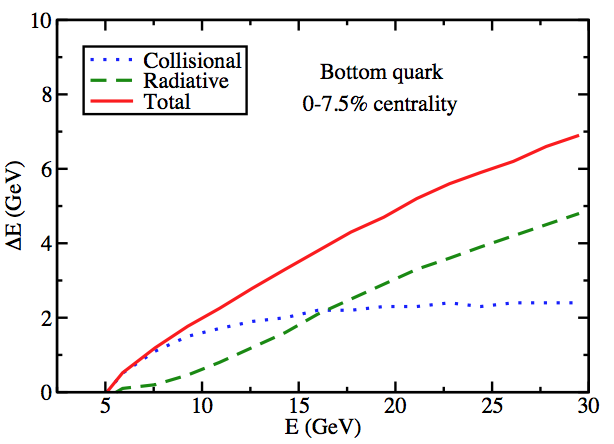
\includegraphics[width=7cm]{FigCap2/HFEnLoss2.png}
  \caption{Comparison of radiative and collisional energy losses for charm (left) and for bottom (right) quarks~\cite{Cao:2013ita}.}
  \label{fig:HFEnLoss}
\end{figure}
In Fig.~\ref{fig:HFEnLoss} the energy loss of charm (left) and beauty (right) quarks 
in central Pb-Pb collisions at the LHC is shown as a function of the initial energy of the quark.
Both the contributions from collisional and radiative energy loss are calculated. Elastic interactions
dominate the low-$\pt$ region, up to $\sim 6\; \Gevc$ for charm and $\sim 16 \;\Gevc$ for beauty quarks.
At higher $\pt$, the contribution from radiative processes is the dominant one and must be considered when 
performing calculations at LHC energies.
It is also interesting to look at Fig.~\ref{fig:HFEnLoss2} (left), that shows the thermalisation process of charm quarks in a static medium with a temperature
$T = 300$ MeV as a function of time, according to the Langevin equation where an additional term for radiative contribution has been added. 
The initial energy of the charm quarks is 10 GeV. Depending on the different implementation for energy
loss, the thermalisation of the charm quarks occurs at different times.\\
\begin{figure}[!ht]
  \centering
  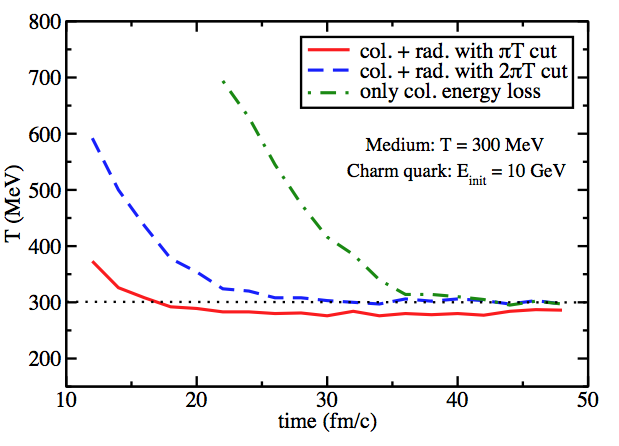
\includegraphics[width=7cm]{FigCap2/HFEnLoss3.png}
  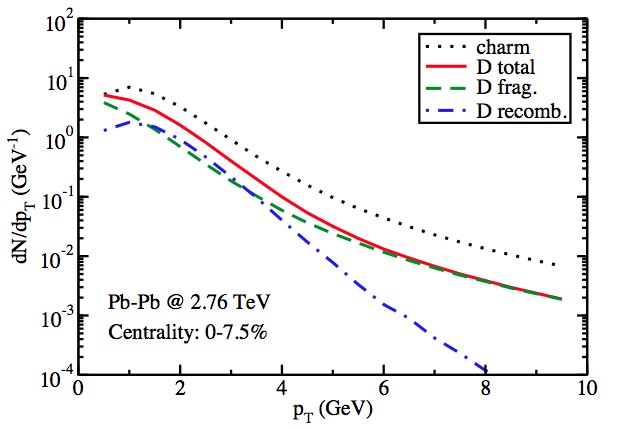
\includegraphics[width=7cm]{FigCap2/FragHQ.png}
  \caption{Left: thermalization process of charm quarks in a static medium~\cite{Cao:2013ita}. Right: relative contributions from different hadronisation mechanisms to D-meson production from charm quarks~\cite{Cao:2013ita}.}
  \label{fig:HFEnLoss2}
\end{figure}
The final hadron yield depends not only on the energy loss mechanism of the parton inside the medium,
but also on the way hadronisation occurs. There are basically two mechanisms for heavy quarks 
to produce heavy flavour hadrons: fragmentation of a high-momentum heavy quark into lower-momentum
hadrons, or coalescence (re-combination) of low-momentum quarks with lighter partons from the thermalised
medium. Fig.~\ref{fig:HFEnLoss2} (right) illustrates the contributions of coalescence and fragmentation 
mechanisms into the final D meson yields from charm quark hadronisation. The ri-combination mechanisms
gives an important contribution at low $\pt$, while the usual fragmentation scenario dominates at higher $\pt$.
Since the coalescence with thermalised lighter partons gives a contribution to the momentum of the 
heavy quark, the $\pt$ distribution of the final hadron will be slightly harder than that of the initial quark,
i.e. shifted towards higher momenta.\\

\begin{figure}[!ht]
  \centering
    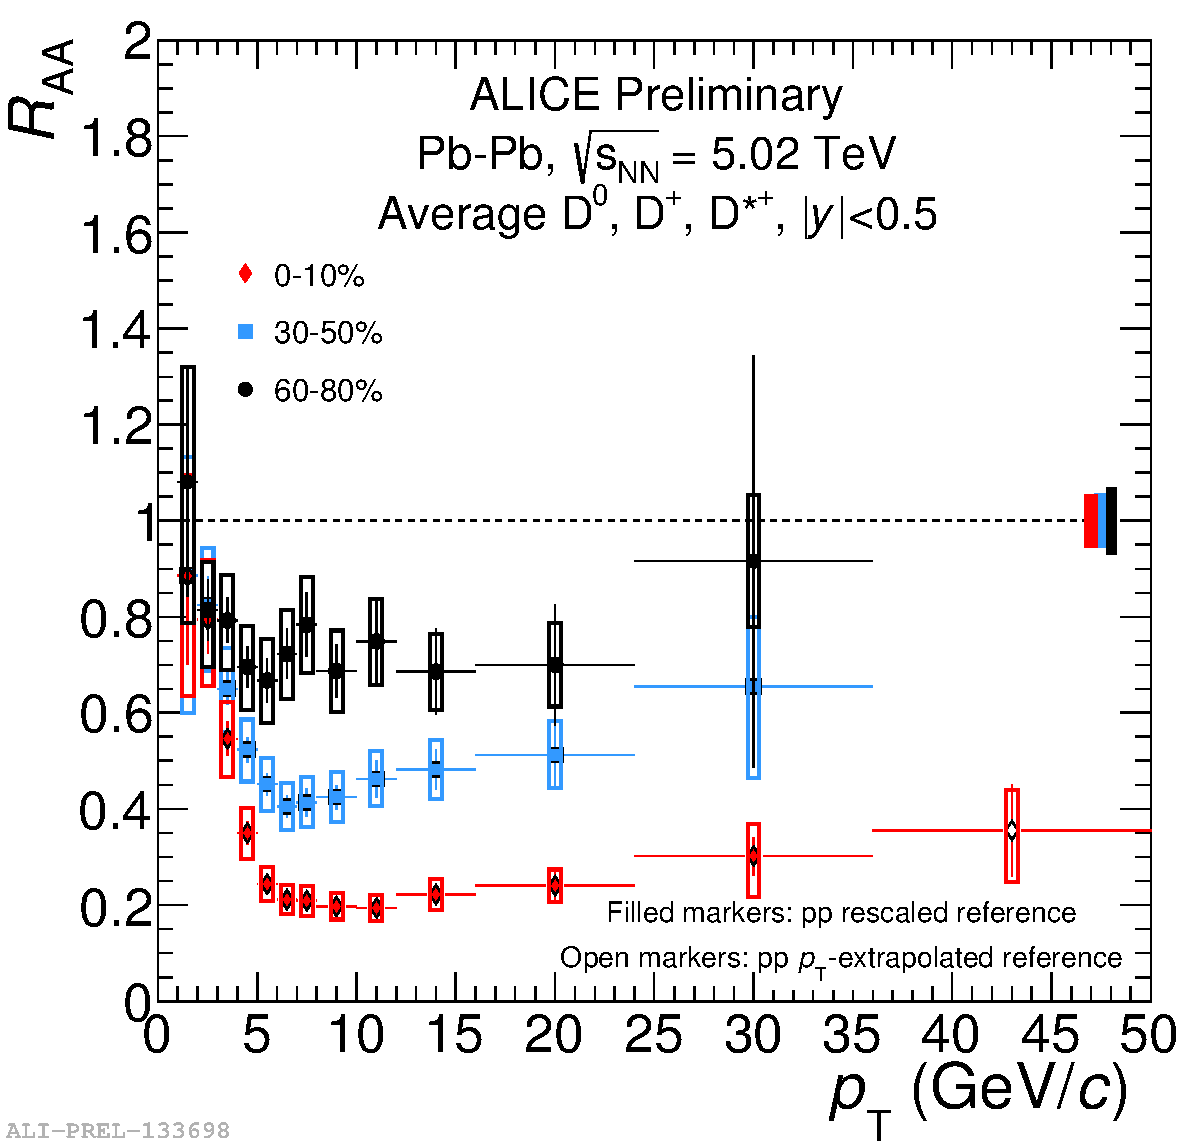
\includegraphics[width=7cm]{FigCap2/2017-Jul-05-DmesonAverage_010_3050_6080_comparison_04July2017.pdf}
  \caption{Average $\RAA$ 
  of prompt $\Dzero$, $\Dplus$ and $\Dstar$ mesons in the 0--10\% (red), 30--50\% (blue) and 60--80\% (black) centrality classes at $\sqrtsNN=5.02~\tev$~\cite{ALICE-PUBLIC-2017-003}. }
  \label{fig:Raa}
\end{figure}

The average nuclear modification factors of $\Dzero$, $\Dplus$ and $\Dstar$ as a function of
$\pt$, in Pb-Pb collisions at $\sNN = 5.02 $ TeV, for the 0--10\%, 30--50\% and 60--80\% centrality classes,
is shown in Fig.~\ref{fig:Raa} (left)~\cite{ALICE-PUBLIC-2017-003}. It shows a suppression that is
maximal at $\pt=6$--$10~\gev/c$ for central and semi-central events, where a reduction of the yields by
a factor of about 5 and 2.5 with respect to the binary-scaled pp reference is observed 
in the two centrality classes, respectively.
The suppression decreases with decreasing $\pt$ for $\pt<6~\GeV/c$, and 
$\RAA$ is compatible with unity  in the interval $1<\pt<3~\gev/c$.
The average $\RAA$ in the 60--80\% centrality class shows a suppression by about 20--30\%, without a pronounced dependence on $\pt$.\\


Fig.~\ref{fig:ColorMassDep} (left) shows the average of the $\Dzero$, $\Dplus$ and $\Dstar$ 
nuclear modification factors as a function of centrality, for the interval 8 $< \pt < 16$ $\Gevc$~\cite{Adam:2015nna}, 
compared with the $\RAA$ of charged pions~\cite{Abelev:2014laa} with $|y| < 0.8$ for the same $\pt$ interval, 
and of non-prompt J$/\psi$ mesons measured by the CMS Collaboration for 6.5 $< \pt < 30$ $\Gevc$ 
in $|y| < 1.2$~\cite{Khachatryan:2016ypw}. The different width of the rapidity interval for D and non-prompt
J$/\psi$ mesons ($|y| < 0.5$ and $|y| < 1.2$, respectively) is not expected to play a big role, since
the intervals are partially overlapping and there is no significant $y$ dependence of the $\RAA$ of 
non-prompt J$/\psi$ mesons in $|y| < 1.2$~\cite{Khachatryan:2016ypw}. The nuclear modification 
factors of charged pions and D mesons are compatible within uncertainties
in all centrality classes. The interpretation of a similar suppression for D mesons and pions is not
straightforward. In the presence of a colour-charge and quark-mass dependent 
energy loss, the harder $\pt$ distribution and the harder fragmentation function of 
charm quarks compared to those of light quarks and gluons could lead to similar 
values of D-meson and pion $\RAA$, as discussed in~\cite{Djordjevic:2013pba}. 
The value of the D-meson $\RAA$ in all the centrality
classes except the most peripheral is lower than that of non-prompt J$/\psi$ mesons. \\
The $\RAA$ of electrons from beauty-hadron decays~\cite{Adam:2016wyz} is compared with the one from charm- and
beauty-hadron decays in Fig.~\ref{fig:ColorMassDep} (right) for the 20\% most central Pb-Pb collisions
~\cite{Adam:2016khe}. The measurements agree within uncertainties at high $\pt$, while in the $\pt$ 
interval 3 $< \pt < 6$ $\Gevc$, the suppression of the $\RAA$ for electrons from beauty-hadron decays 
is about 1.2$\sigma$ less. This difference is consistent with what explained above for the comparison of prompt D meson 
and J$/\psi$ from B meson. The observation of different suppression for particles originating from
charm or beauty quarks is consistent with theoretical calculations in which in-medium parton energy loss 
decreases with increasing quark mass.
\begin{figure}[!ht]
  \centering
    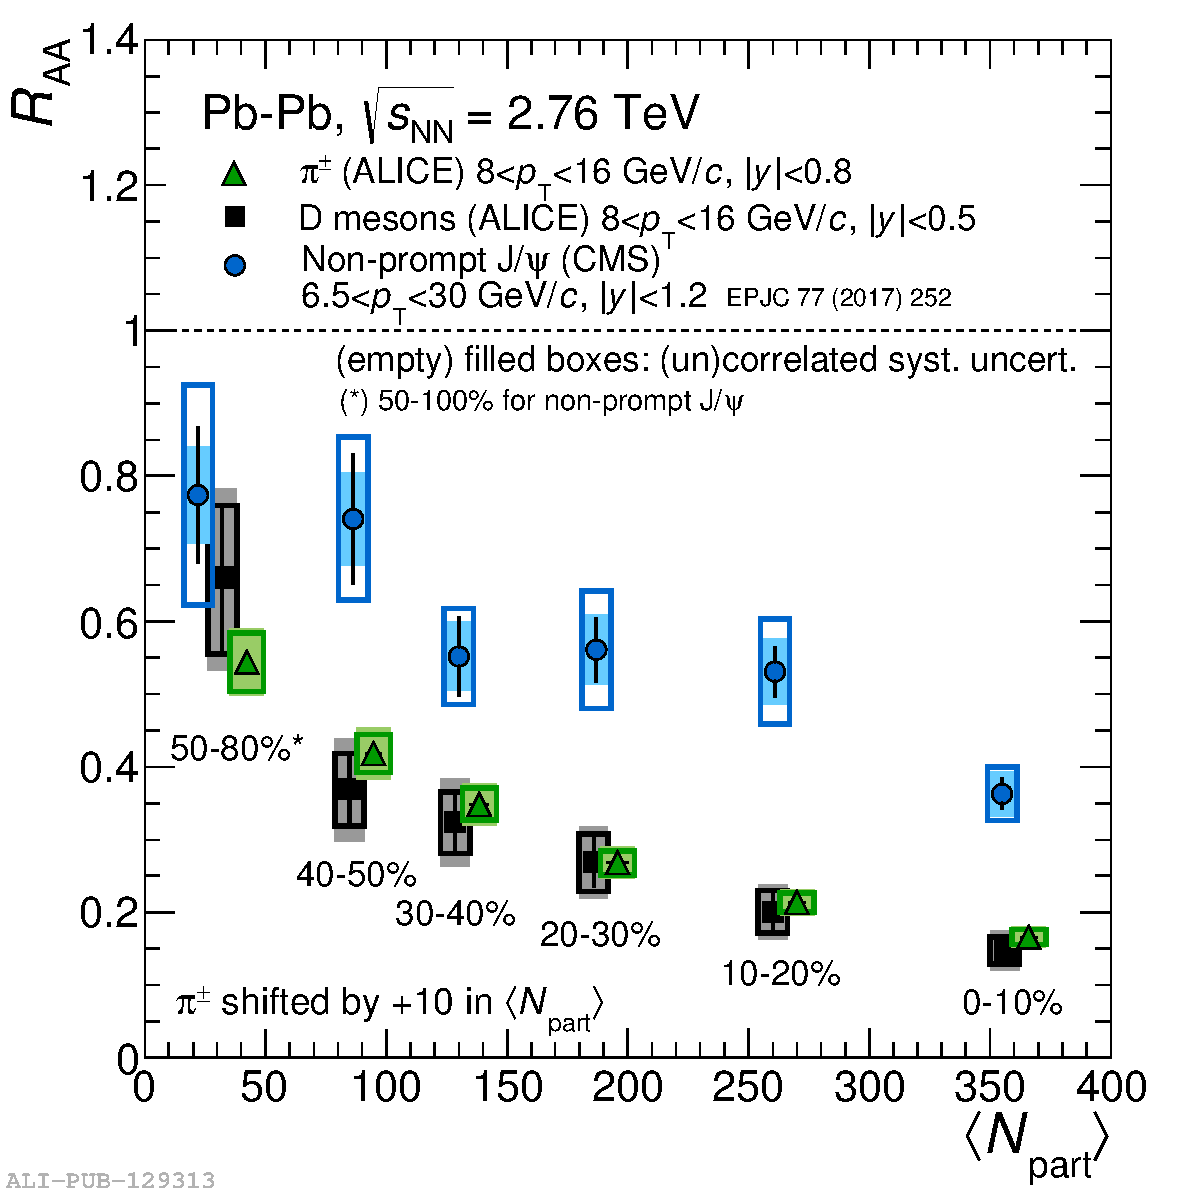
\includegraphics[width=7cm]{FigCap2/2017-May-22-RaavsNpart_Dmes8to16_Pions8to16_FinalNonPromptJpsi2017_CC_25042017.pdf}
    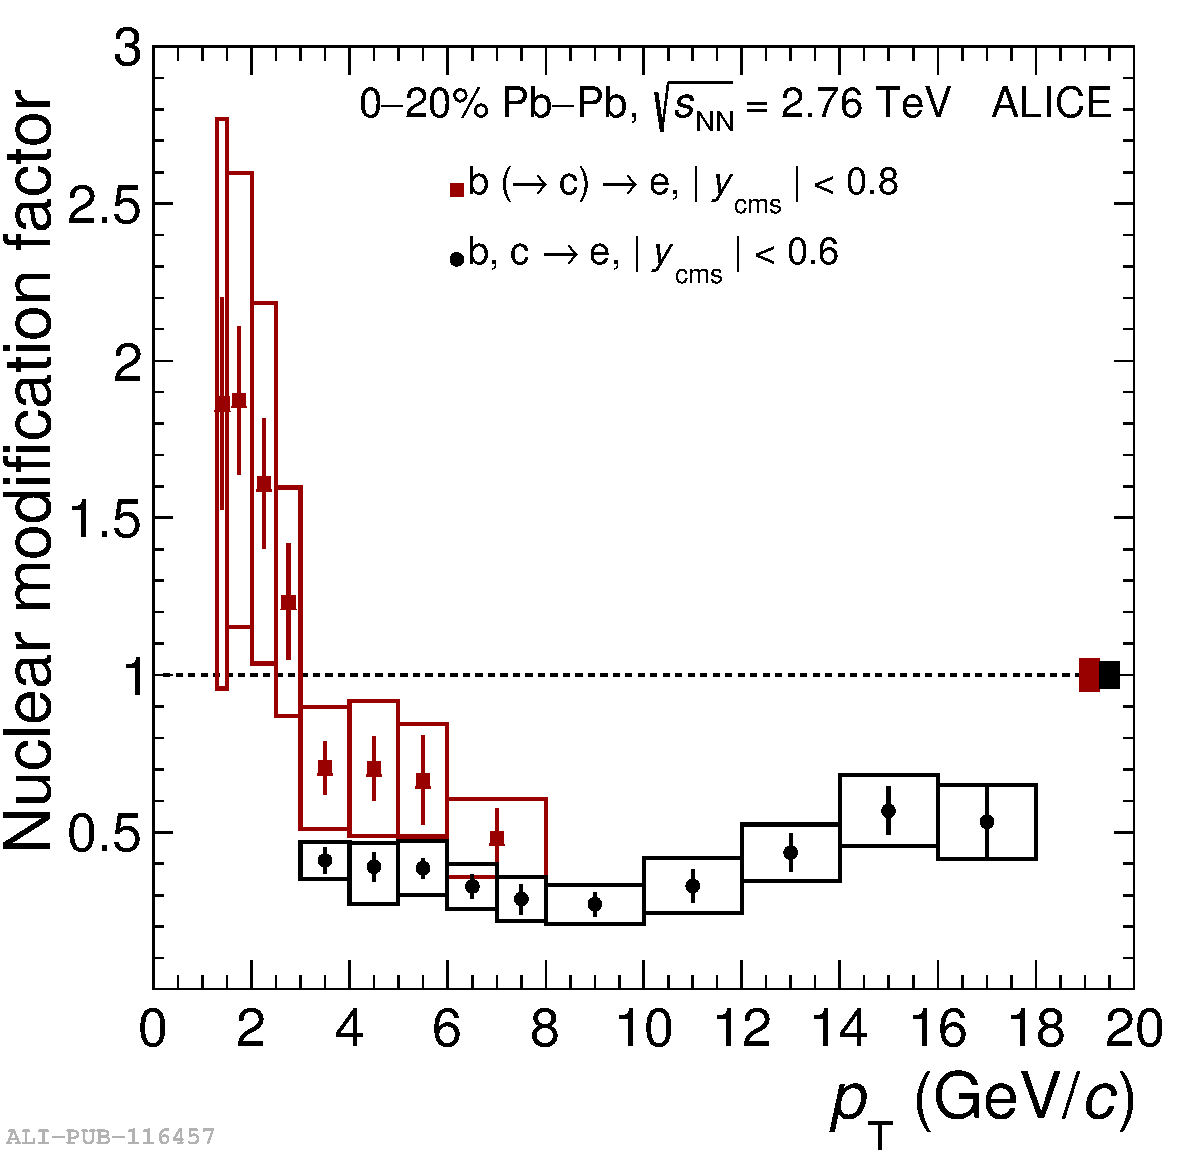
\includegraphics[width=7cm]{FigCap2/2017-Jan-28-rParAAbeautyincl.pdf}
  \caption{Left: Comparison of the D-meson~\cite{Adam:2015nna} and charged-pion~\cite{Abelev:2014laa} $\RAA$ in 8 $< \pt < 16$ $\Gevc$~\cite{Adam:2015nna} 
and of the $\RAA$ of non-prompt J$/\psi$ mesons in 6.5 $< \pt < 30$ $\Gevc$ measured by CMS~\cite{Khachatryan:2016ypw}. 
Right: $\RAA$ of electrons from beauty-hadron decays together with
the corresponding result for beauty- and charm-hadron decays~\cite{Adam:2016khe} for the 20\% most central Pb-Pb collisions.}
  \label{fig:ColorMassDep}
\end{figure}

\begin{figure}[!ht]
  \centering
        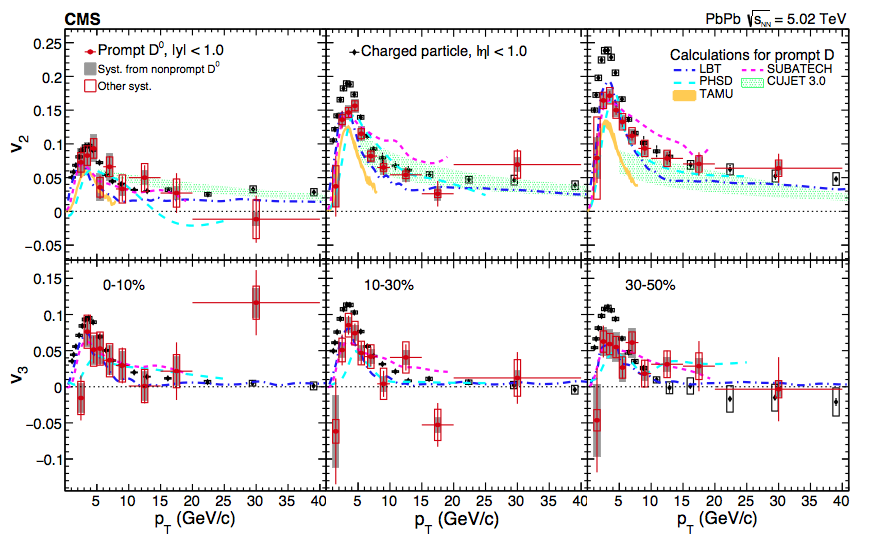
\includegraphics[width=14cm]{FigCap2/D0v2_CMS_5TeV.png}
  \caption{Prompt $\Dzero$ meson $v_2$ (upper) and $v_3$ (lower) coefficients at midrapidity ($|y| < 1.0$) for
the centrality classes 0-10\% (left), 10-30\% (middle), and 30-50\% (right)~\cite{Sirunyan:2017plt}.}
  \label{fig:D0v2CMS}
\end{figure}

The $v_2$ and $v_3$ of prompt $\Dzero$ meson measured by CMS at $\sNN = 5.02 $ TeV in the 0-10\%, 
10-30\% and ?30-50\% classes are in Fig.~	\ref{fig:D0v2CMS}~\cite{Sirunyan:2017plt}. The measured $v_2$ and $v_3$ are larger than 0 
at low $\pt$, to decrease than at higher $\pt$.
This result, in agreement with what observed by ALICE~\cite{Acharya:2017qps}, suggests that charm quarks take part in 
the collective motion of the medium and that collisional interaction processes as well as quark 
recombination may contribute to the observed elliptic flow. \\

The simultaneous comparison of $\RAA$ and elliptic flow $v_2$ measurements at $\sqrtsNN=5.02~\tev$~\cite{Acharya:2017qps} with models can provide more stringent constraints to the implementation of the interaction and hadronisation processes for heavy quarks. 
This comparison is shown in Fig.~\ref{RAAandv2} for the $\RAA$  
and $v_2$, in the 0--10\% and 30--50\% centrality classes respectively, together with models that provide simultaneous description of the observables.
The level of model-to-data consistency was quantified in terms of the reduced $\chi^2$ in the respective $\pt$ interval where the calculations are available.
Values of reduced $\chi^2$ for $\RAA$ measurements in 0--10\% and 30--50\% centrality classes and $v_2$ in 30--50\% centrality class are reported in Table~\ref{tab:RedChi2}.
TAMU model overestimates $\RAA$ at high $\pt$ in central events and describes the magnitude of the elliptic flow, but fails in reproducing the shape.
BAMPS-el overestimates the maximum flow while underestimating the suppression at high $\pt$. The radiative term in BAMPS-el+rad improves the description of the $\RAA$ but gives a smaller than observed maximum $v_2$.~PHSD, POWLANG, LBT and MC@sHQ provide instead a fair description of both $v_2$ magnitude and shape
as well as of energy loss, as their values of $\chi^2/$ndf indeed show. 





\begin{figure}[!ht]
  \centering
    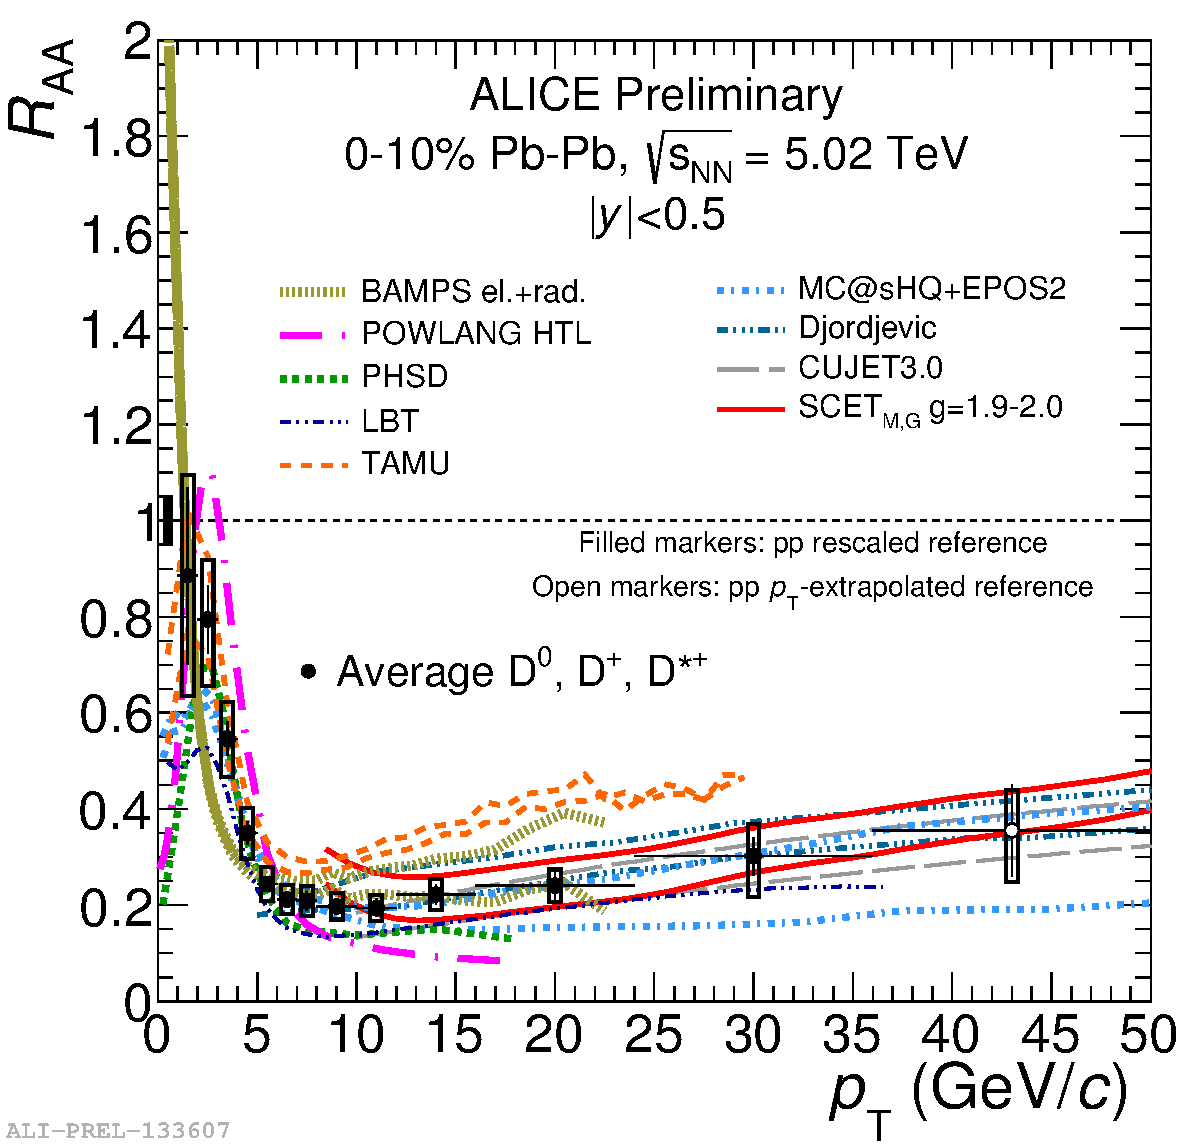
\includegraphics[width=7cm]{FigCap2/2017-Jul-07-DmesonAverage_010_All_Models_04July2017.pdf}
    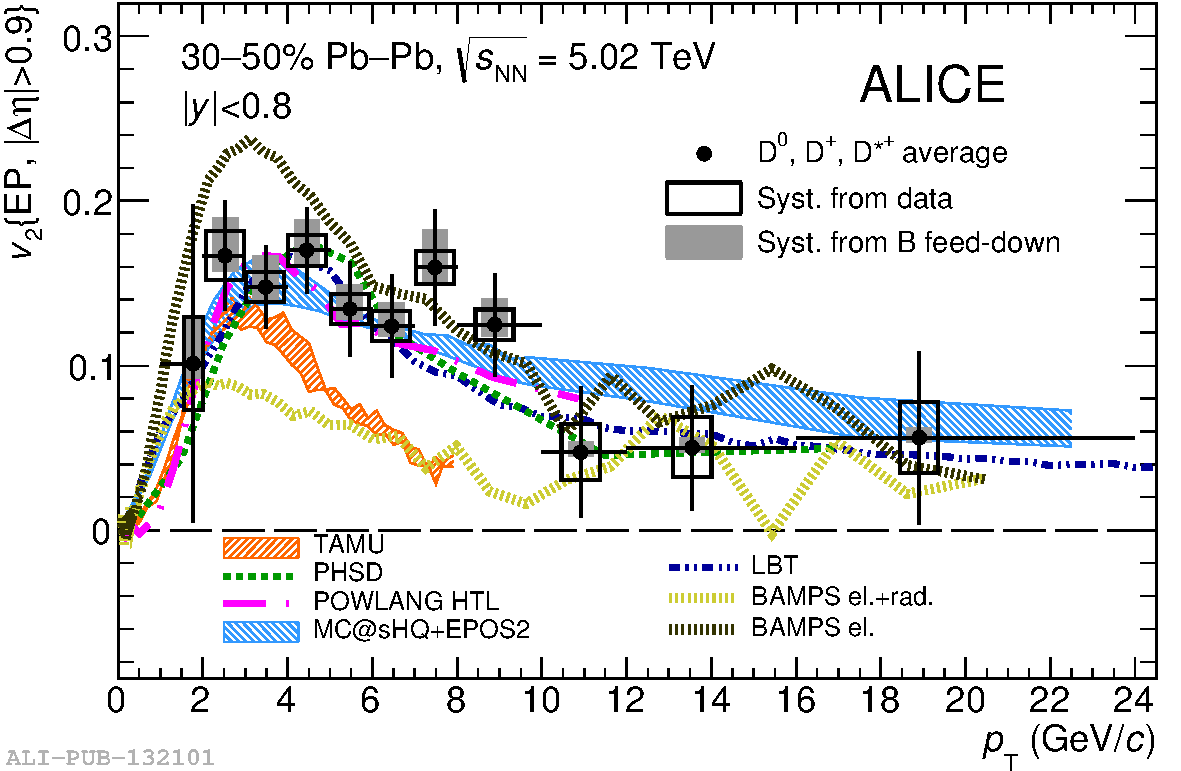
\includegraphics[width=7cm]{FigCap2/2017-Jul-04-DmesonComparisonWithModels.pdf}
%    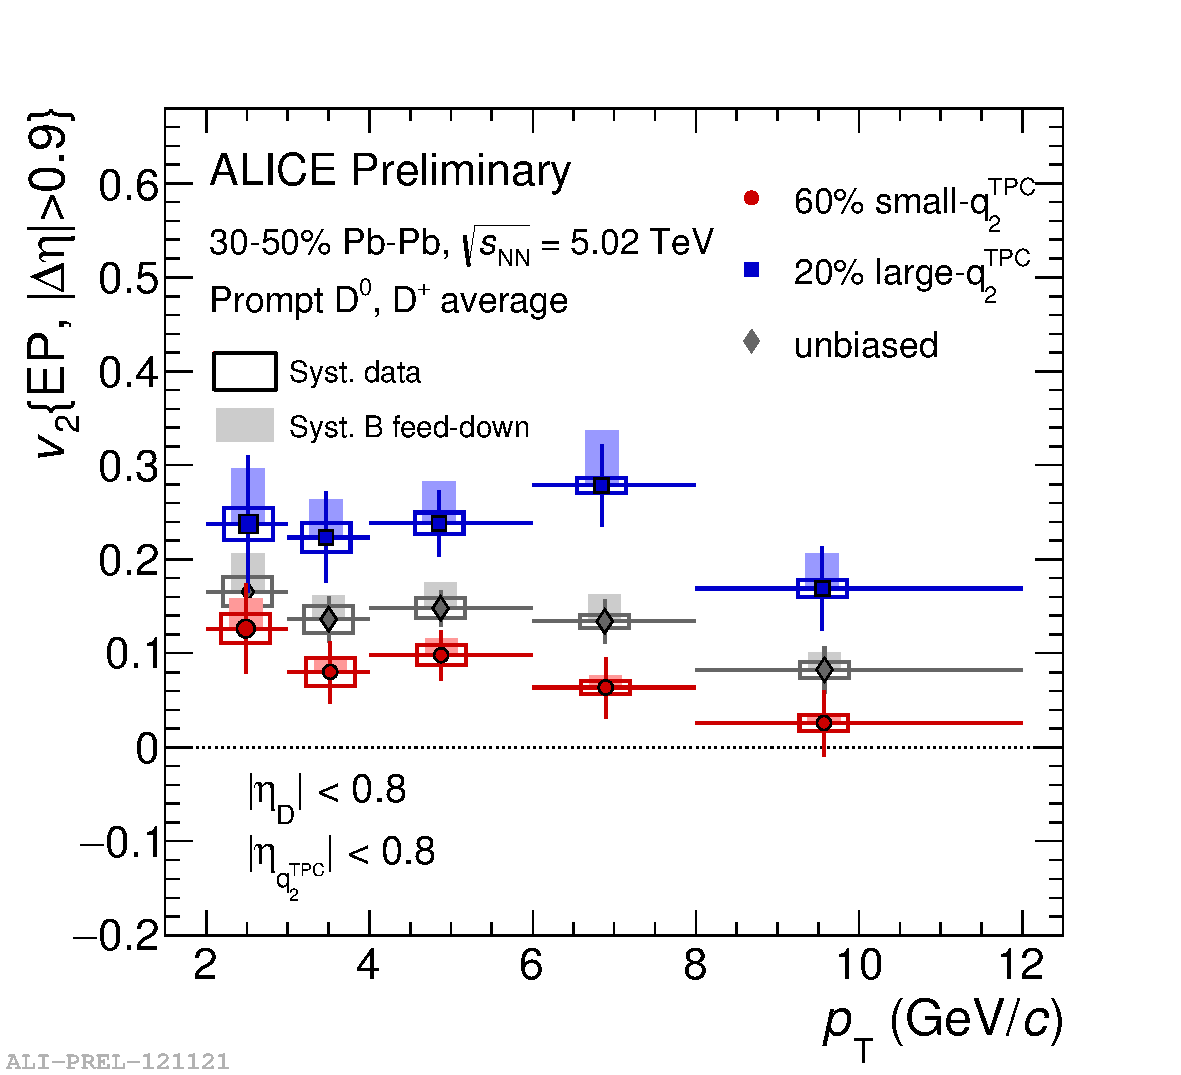
\includegraphics[width=7cm]{FigCap2/2017-Sep-13-v2ESE_Daverage_PbPb3050_VZERO_q2TPCFullSmall60Perc_q2TPCFullLarge20perc.pdf}
  \caption{Left: average D-meson $\RAA$ in the 0--10\% centrality class compared with models~\cite{ALICE-PUBLIC-2017-003}.}
  \label{fig:}
\end{figure}

Models provide:
Diffusion coefficient 2$\pi T D_s(T) \approx 1.5-7$ at critical temperature Tc
Charm thermalization time tcharm $\sim 3-14$ fm/c

 By comparing different models to experimental data from CMS [45] and ALICE [52] values of the
transport coefficient ?q ? 1.7?1.9 GeV2
/c were extracted [64, 65]
